\documentclass[10pt,twocolumn,twoside]{IEEEtran}
%\documentclass[11pt,draftcls,onecolumn]{IEEEtran} 
% *** CITATION PACKAGES ***
\usepackage{cite}

% *** GRAPHICS RELATED PACKAGES ***
\usepackage{graphicx}
\graphicspath{{./images/}}
\DeclareGraphicsExtensions{.eps}
\usepackage[update,prepend]{epstopdf}
%\usepackage{caption}% http://ctan.org/pkg/caption


% *** MATH PACKAGES ***
\usepackage[cmex10]{amsmath}
\usepackage{mathrsfs} %草寫體數學符號,在數學模式裡用 \mathscr{E} 得草寫 E
\interdisplaylinepenalty=2500

% *** SUBFIGURE PACKAGES ***
\usepackage[caption=false,font=footnotesize]{subfig}

% *** ALIGNMENT PACKAGES ***
%
\usepackage{array}


% *** FLOAT PACKAGES ***
\usepackage{dblfloatfix}



% correct bad hyphenation here
\hyphenation{op-tical net-works semi-conduc-tor}
\newcommand{\argmin}{\operatornamewithlimits{arg\ min}}

\begin{document}



% paper title
\title{Iterative 3D-MRF based Decoder \\ for Uncompressed Wireless Video Transmission}


\author{ Kuan-Yu Lin , Wei-Chih Hung, Bai-Xi Li , Ping-Cheng Yeh \\
National Taiwan University}% <-this % stops a space

% note the % following the last \IEEEmembership and also \thanks - 
% these prevent an unwanted space from occurring between the last author name
% and the end of the author line. i.e., if you had this:
% 
% \author{....lastname \thanks{...} \thanks{...} }
%                     ^------------^------------^----Do not want these spaces!
%
% a space would be appended to the last name and could cause every name on that
% line to be shifted left slightly. This is one of those "LaTeX things". For
% instance, "\textbf{A} \textbf{B}" will typeset as "A B" not "AB". To get
% "AB" then you have to do: "\textbf{A}\textbf{B}"
% \thanks is no different in this regard, so shield the last } of each \thanks
% that ends a line with a % and do not let a space in before the next \thanks.
% Spaces after \IEEEmembership other than the last one are OK (and needed) as
% you are supposed to have spaces between the names. For what it is worth,
% this is a minor point as most people would not even notice if the said evil
% space somehow managed to creep in.



% The paper headers
%\markboth{Journal of \LaTeX\ Class Files,~Vol.~11, No.~4, December~2012}%
%{Shell \MakeLowercase{\textit{et al.}}: Bare Demo of IEEEtran.cls for Journals}
% The only time the second header will appear is for the odd numbered pages
% after the title page when using the twoside option.
% 
% *** Note that you probably will NOT want to include the author's ***
% *** name in the headers of peer review papers.                   ***
% You can use \ifCLASSOPTIONpeerreview for conditional compilation here if
% you desire.




% If you want to put a publisher's ID mark on the page you can do it like
% this:
%\IEEEpubid{0000--0000/00\$00.00~\copyright~2012 IEEE}
% Remember, if you use this you must call \IEEEpubidadjcol in the second
% column for its text to clear the IEEEpubid mark.



% use for special paper notices
%\IEEEspecialpapernotice{(Invited Paper)}


% make the title area
\maketitle

% As a general rule, do not put math, special symbols or citations
% in the abstract or keywords.
\begin{abstract}
Due to the emergence of mmWave systems that provide multi-Gbps data rate over 60GHz band, uncompressed video transmission has been considered as a commonly used feature for wireless multimedia transmission over the wireless personal area networks (WPANs). However, mmWaves signals usually have higher attenuation than the conventional low-frequency wireless signals, and therefore supporting transmission in a low SNR condition becomes a challenging problem for such systems. In this paper, we propose a 3D-MRF model and an iterative source-channel decoding method based on the proposed 3D-MRF model for the wireless transmission of uncompressed video. With our proposed iterative decoding structure, the video decoder utilizes the temporal and spatial redundancy among the video frames to jointly decode the received coded bits with the aid of 3D-MRF model. The numerical results show that the proposed method can significantly enhance the video quality in terms of PSNR, even while operating in an extremely low SNR condition. 
\end{abstract}

% Note that keywords are not normally used for peerreview papers.
\begin{IEEEkeywords}
Markov random fields, iterative source-channel decoding, wireless communication, video signal processing.
\end{IEEEkeywords}



% For peer review papers, you can put extra information on the cover
% page as needed:
% \ifCLASSOPTIONpeerreview
% \begin{center} \bfseries EDICS Category: 3-BBND \end{center}
% \fi
%
% For peerreview papers, this IEEEtran command inserts a page break and
% creates the second title. It will be ignored for other modes.
\IEEEpeerreviewmaketitle



\section{Introduction}

\begin{figure*}[!t]
	\centering
	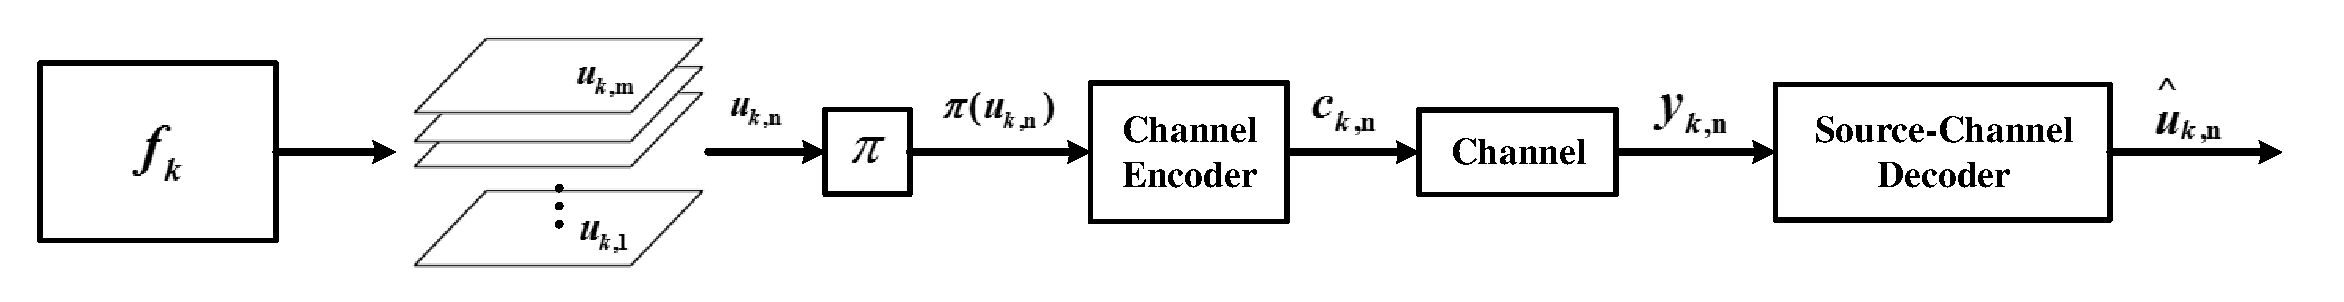
\includegraphics[width=\textwidth]{sm.pdf}
	\caption{Wireless video transmission model.}
\label{trans_model}
\end{figure*}

\IEEEPARstart{T}{he}  prevalence of video technology make it easy for people to access multimedia services and products such as digital films, video streaming and Internet video communications. Recently, due to the emergence of mmWave systems that provide multi-Gbps data rate over 60GHz band, the video transmission systems using Ultra-wideband (UWB) techniques for the emerging wireless personal area networks (WPANs), such as WirelessHD \cite{WirelessHD} and Wireless Gigabit Alliance \cite{Wigig}, have been developed for better user experience. Different from conventional video streaming systems, these systems require low latency and lossless video quality in order to support features such as display and user interaction. Also, in WPANs the video sources are typically uncompressed HDMI streams from game consoles, PCs and mobile devices. Therefore, with the aid of multi-Gbps data rate over 60GHz band, video sequences are usually transmitted without compression in WPANs video transmission systems \cite{60ghz}.

When transmitting over such high-frequency band, wireless signals tends to be much more fragile, compared to the conventional low-frequency wireless signals. In other words, uncompressed video transmission systems over high-frequency band could operate in a low signal-to-noise ratio (SNR) condition, and it might results in damaged video frames. There are several works providing different solutions to enhance the video quality in an uncompressed video transmission system. In \cite{60ghz}, pixel partitioning and uncompressed automatic repeat request (UV-ARQ) are proposed. Unequal error protection (UEP), in which different modulation and coding schemes (MCs) are imposed to different pixel levels, is adopted in both \cite{60ghz} and \cite{ucp_v}. Furthermore, since in uncompressed video transmission neither the spatial nor the temporal redundancy is removed from the video source, joint source-channel coding (JSCC) \cite{JSCC} can be performed to exploit the redundancy. The question of redundancy reuse is similar to the classic Slepian-Wolf theorem \cite{sw}, which states that the achievability of the sum-rate of the separated lossless compression of the two correlated sources can be equal to the joint entropy. However, in JSCC, the correlations are not used to compress the sources but used to improve the communication reliability. By combing the side information along with error correction code, a communication system can achieve better performance than the one without utilizing the side information. In \cite{JSCC_SCCD} and \cite{softbit}, JSCC is used for speech error concealment with the aid of first-order Markov process. 

Based on JSCC, iterative source-channel decoding (ISCD) \cite{ISCD, ISCD2, ISCD3, ISCD4, ISCD5} was developed as a turbo-like \cite{turbocode} decoding structure to exchange the extrinsic information between channel decoder and source decoder, and thus increasing the error robustness of the receiver. In \cite{ISCD_image}, ISCD is used for image transmission with the assumption that each image pixel is constrained by two first-order Markov processes in horizontal and vertical directions. The same model is generalized from 2D to 3D by taking the third temporal first-order Markov process in video into consideration in \cite{ISCD_st}. In \cite{ISCD_st}, the state transition probability of the first-order Markov process is obtained by off-line statistic data of videos, and the temporal first-order Markov process is formed by assuming a pixel is related to all pixels in the same location within every video frame. A ISCD scheme for image decoding using Markov Random field (MRF) to model the relationship between neighboring pixels is proposed in \cite{ISCD_MRF} and \cite{ISCD_MRF2}, where the MRF parameter is estimated in encoder and transmitted to the ISCD decoder which consists a channel decoder and an iterative MRF decoder.

In this paper, we propose an iterative source-channel decoding method for uncompressed video transmission based on a proposed novel 3D-MRF model. The 3D-MRF model is a bit-plane level MRF model which successfully reveals the spatial and temporal redundancy of video sequences. For those video sequences of intense movement, we utilize the motion estimation at the decoder side to precisely locate the temporal movement under the block-base view, and thus the temporal redundancy can be fully used by the 3D-MRF. Through the 3D-MRF model, we develop the 3D-MRF based soft-in soft-out (SISO) source decoding algorithm. The 3D-MRF based SISO source decoding algorithm with low complexity while can significantly improves the decoding performance. Based on the 3D-MRF based SISO decoding, we design an iterative source-channel decoding structure which is capable of jointly estimating the MRF parameters at the receiver, and thus the proposed decoder can automatically adjust the amount of the information exchange according to the decoding video sequence. Also, by adding a single buffer into our decoder structure, the temporal extrinsic information is allowed to propagate throughout the video decoding process. We show that the proposed ISCD method can significantly enhance the video quality in terms of peak signal-to-noise ratio (PSNR). Even under very low SNR condition, the video frames are still maintained in good quality. Furthermore, It is worth noting that our proposed decoding method can cooperate with any existing UEP solutions implemented in the transmitter to provide further improvement in video quality.

The content of this paper is organized as follows. In Section \ref{sec_sm} the transmission system and the wireless channel model are introduced. The 3D-MRF model and the 3D-MRF based SISO source decoder is proposed in Section \ref{sec_3dmrf}. The ISCD decoding method with the joint estimation of the 3D-MRF parameter and motion estimation at the decoder side are shown in Section \ref{sec_alg}. The extrinsic information transfer (EXIT) chart analysis of the proposed iterative source-channel decoder is provided in Section \ref{sec_exit}.  The simulation result is shown in Section \ref{sec_exp}. Finally the conclusion is made in Section \ref{sec_con}.

\section{System model} \label{sec_sm}

We consider the wireless video transmission model as depicted in Fig. \ref{trans_model}. At time instant $\tau$, a video frame $F_k$ with incremental index $k$ is captured from the video source. The set consisting of the pixels from $F_k$ is denoted as
\begin{equation}
\mathbf{f}_k = \{f_k^{(x,y)}|x\in\{1,..,w\}, y\in\{1,...,h\}\},
\end{equation} 
where $(w,h)$ are the width and height of the video frame $F_k$. Each element of $\mathbf{f}_k$ is an $m$-bit unsigned integer, whose value ranges from $0$ to $2^m-1$. For convenience, the video frame pixels can also be represented in a bit-plane way, where
\begin{equation}
\mathbf{u}_{k,n} = \{u_{k,n}^{(x,y)} = f_k^{(x,y)}(n) | \forall f_k^{(x,y)} \in \mathbf{f}_k\}
\end{equation} 
are the $n$-th bit-plane of the $k$-th video frame with $n = 1,...,m$, and $f_k^{(x,y)}(n)$ is the $n$-th bit of $f_k^{(x,y)}$ ( $n=1$ for the most significant bit (MSB)  and $n=m$ for the least significant bit (LSB).) Each bit-plane is scanned into serial bit-sequence and interleaved by the block $\pi$ in Fig. \ref{trans_model} which is assumed to be a random interleaver. After applying the channel code on interleaved bit sequence, we obtain the channel-coded bit sequence $\mathbf{c}_{k,n} = [c_{k,n}^1, c_{k,n}^2,...,c_{k,n}^{w\cdot h/R_c}]$ with $w \cdot h$ denoting the total number of bits in a bit-plane and the code rate $R_c$ of the applied channel code. These coded bits are then modulated and passed through an additive white Gaussian noise (AWGN) channel with signal-to-noise ratio (SNR) $E_b/N_0$. Assuming binary phase shift keying (BPSK) is used, the received signal of $c_{k,n}^i$ can be described by
\begin{equation}
y_{k,n}^i = (2c_{k,n}^i - 1) + z, z \sim Gau(0,\frac{N_0}{2\sqrt{E_s}}),
\end{equation}
where $Gau(\mu,\sigma^2)$ is the Gaussian distribution with mean $\mu$ and variance $\sigma^2$. Furthermore, the log-likelihood ratio (LLR) is computed as
\begin{equation}
L(y_{k,n}^i) =\ln[ \frac{p(y_{k,n}^i | c_{k,n}^i = 0)}{p(y_{k,n}^i | c_{k,n}^i = 1)}] = 4\frac{E_s}{N_0}y_{k,n}^i,
\end{equation}
where $p(\cdot)$ is the probability distribution function (p.d.f) of $y_{k,n}^i$. These LLR values are then passed through our proposed 3D-MRF decoder whose output is the estimated source bit sequence $\hat{\mathbf{u}}_{k,n}$.

\begin{figure*}[!t]
	\centering
	\subfloat[]{\label{subfig_3DMRF_s}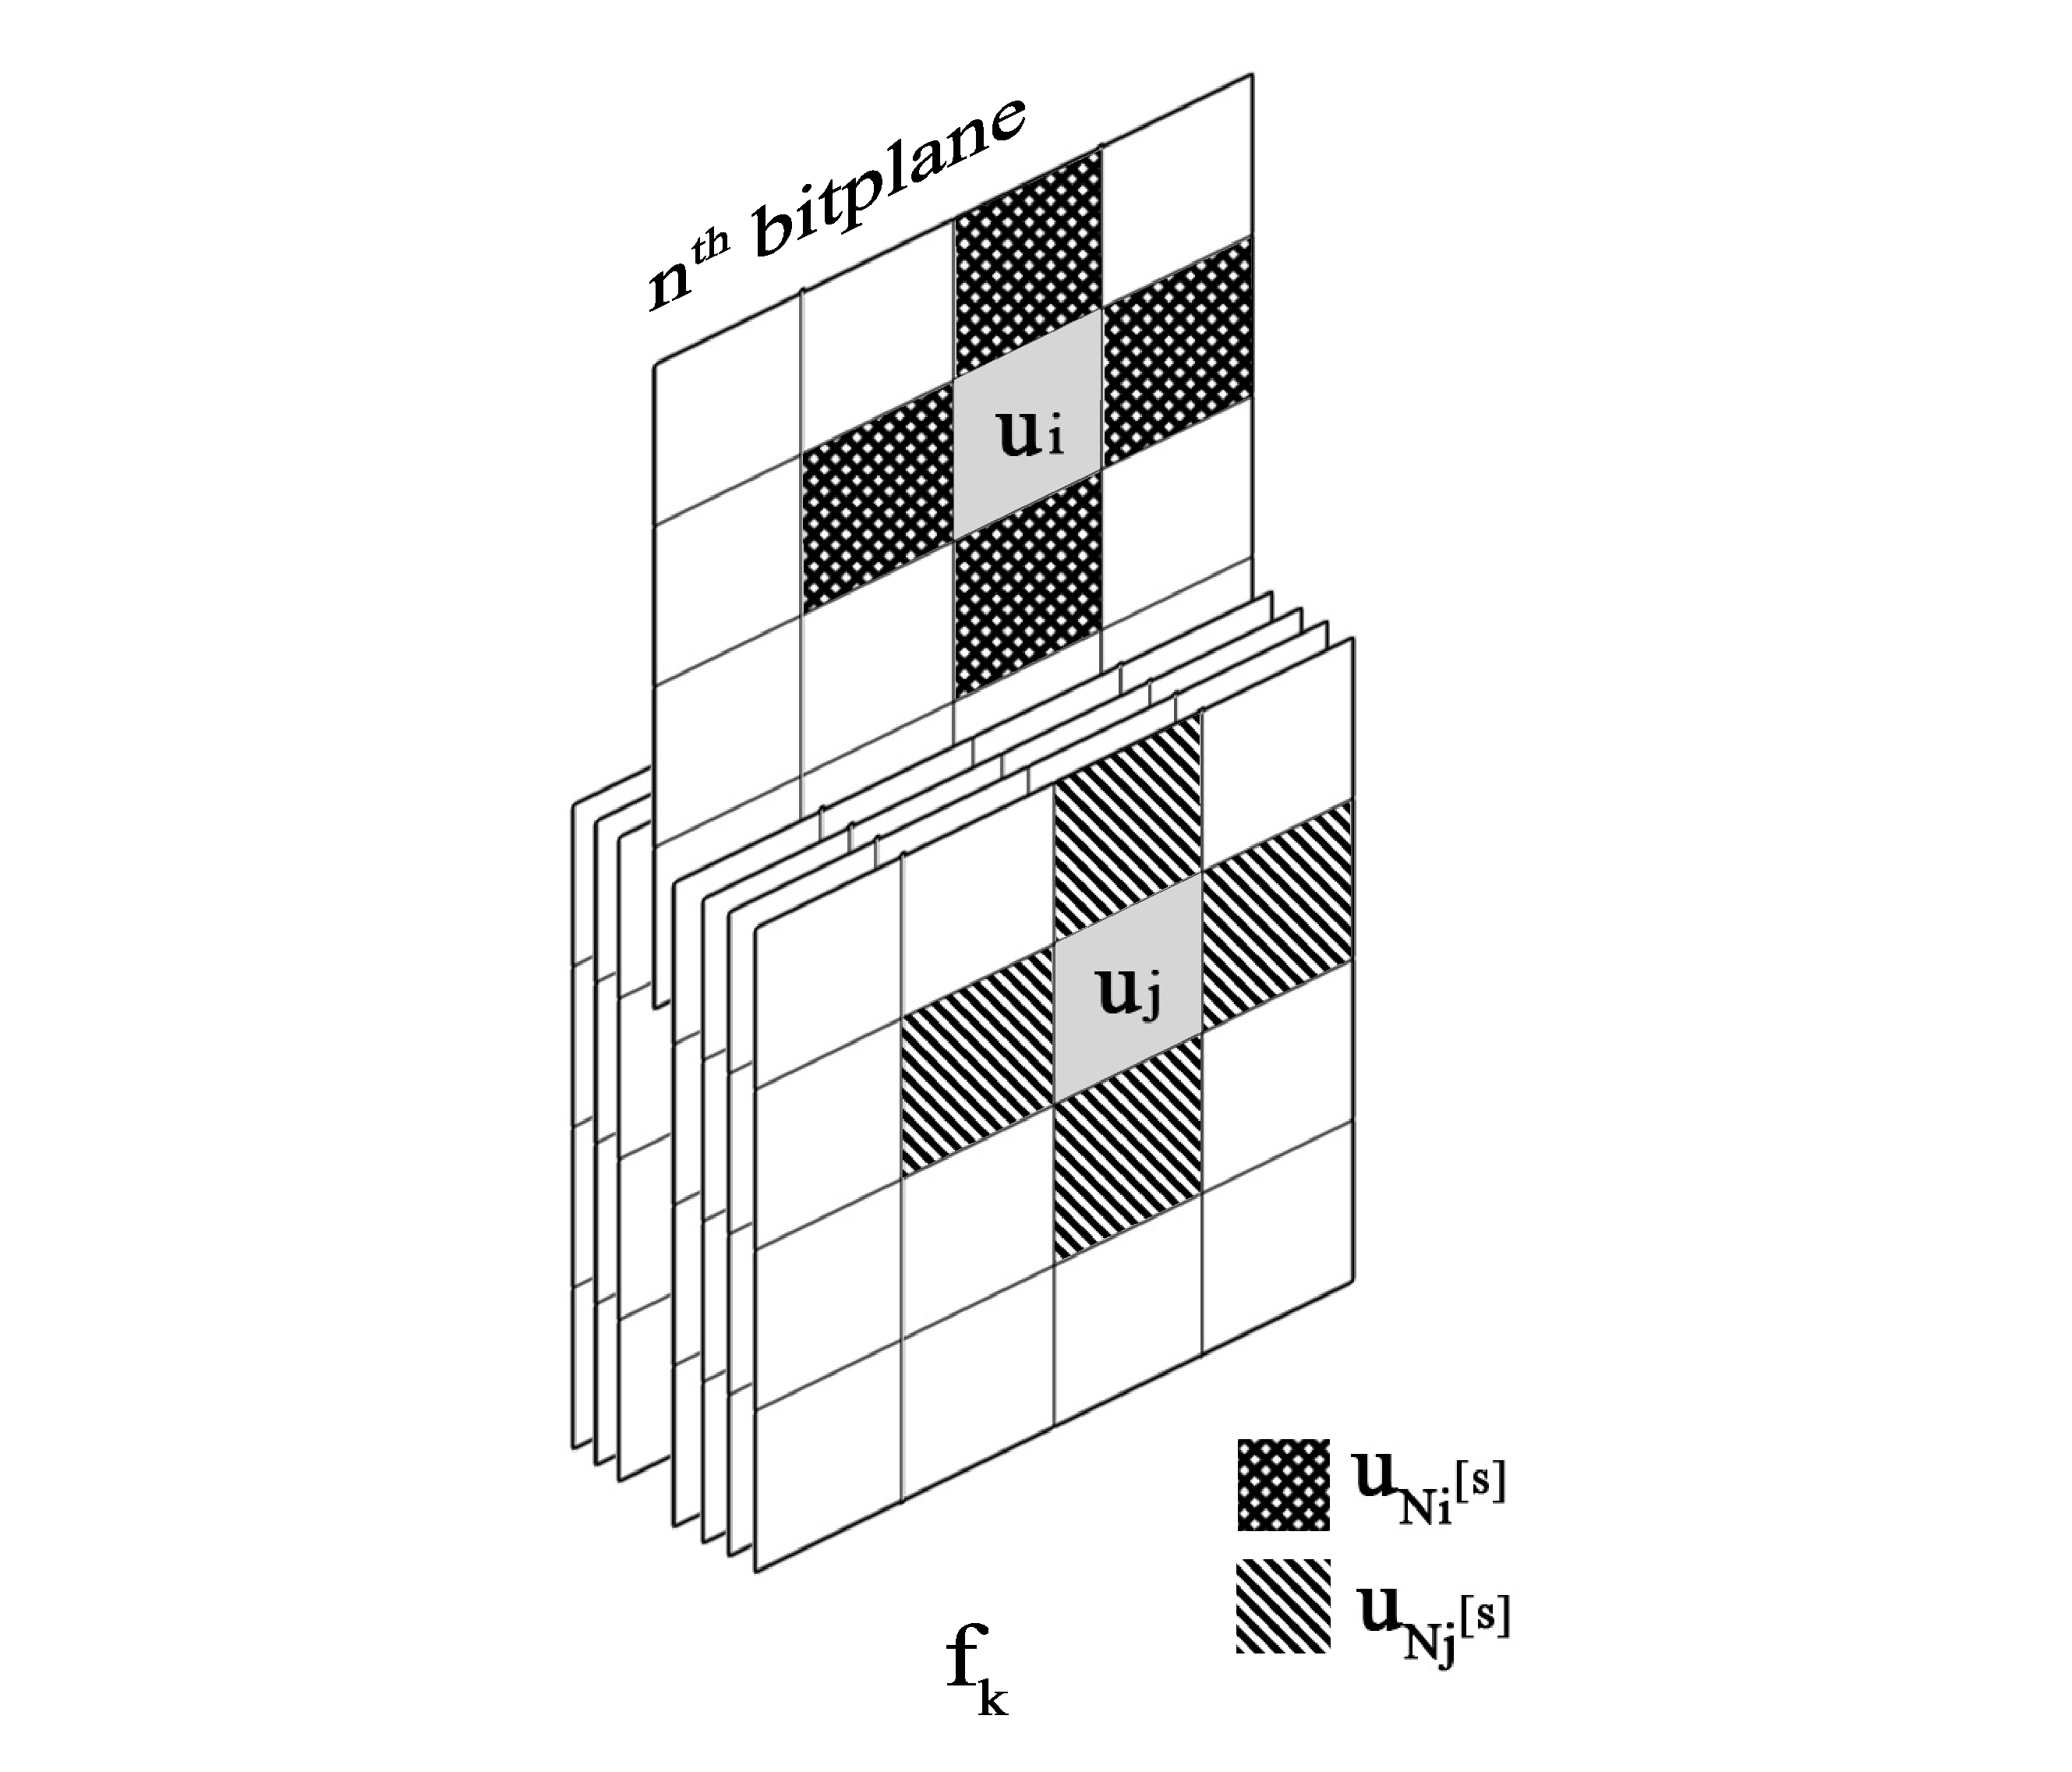
\includegraphics[height=0.25\textheight]{MRF_spatial}} 
	\subfloat[]{\label{subfig_3DMRF_t}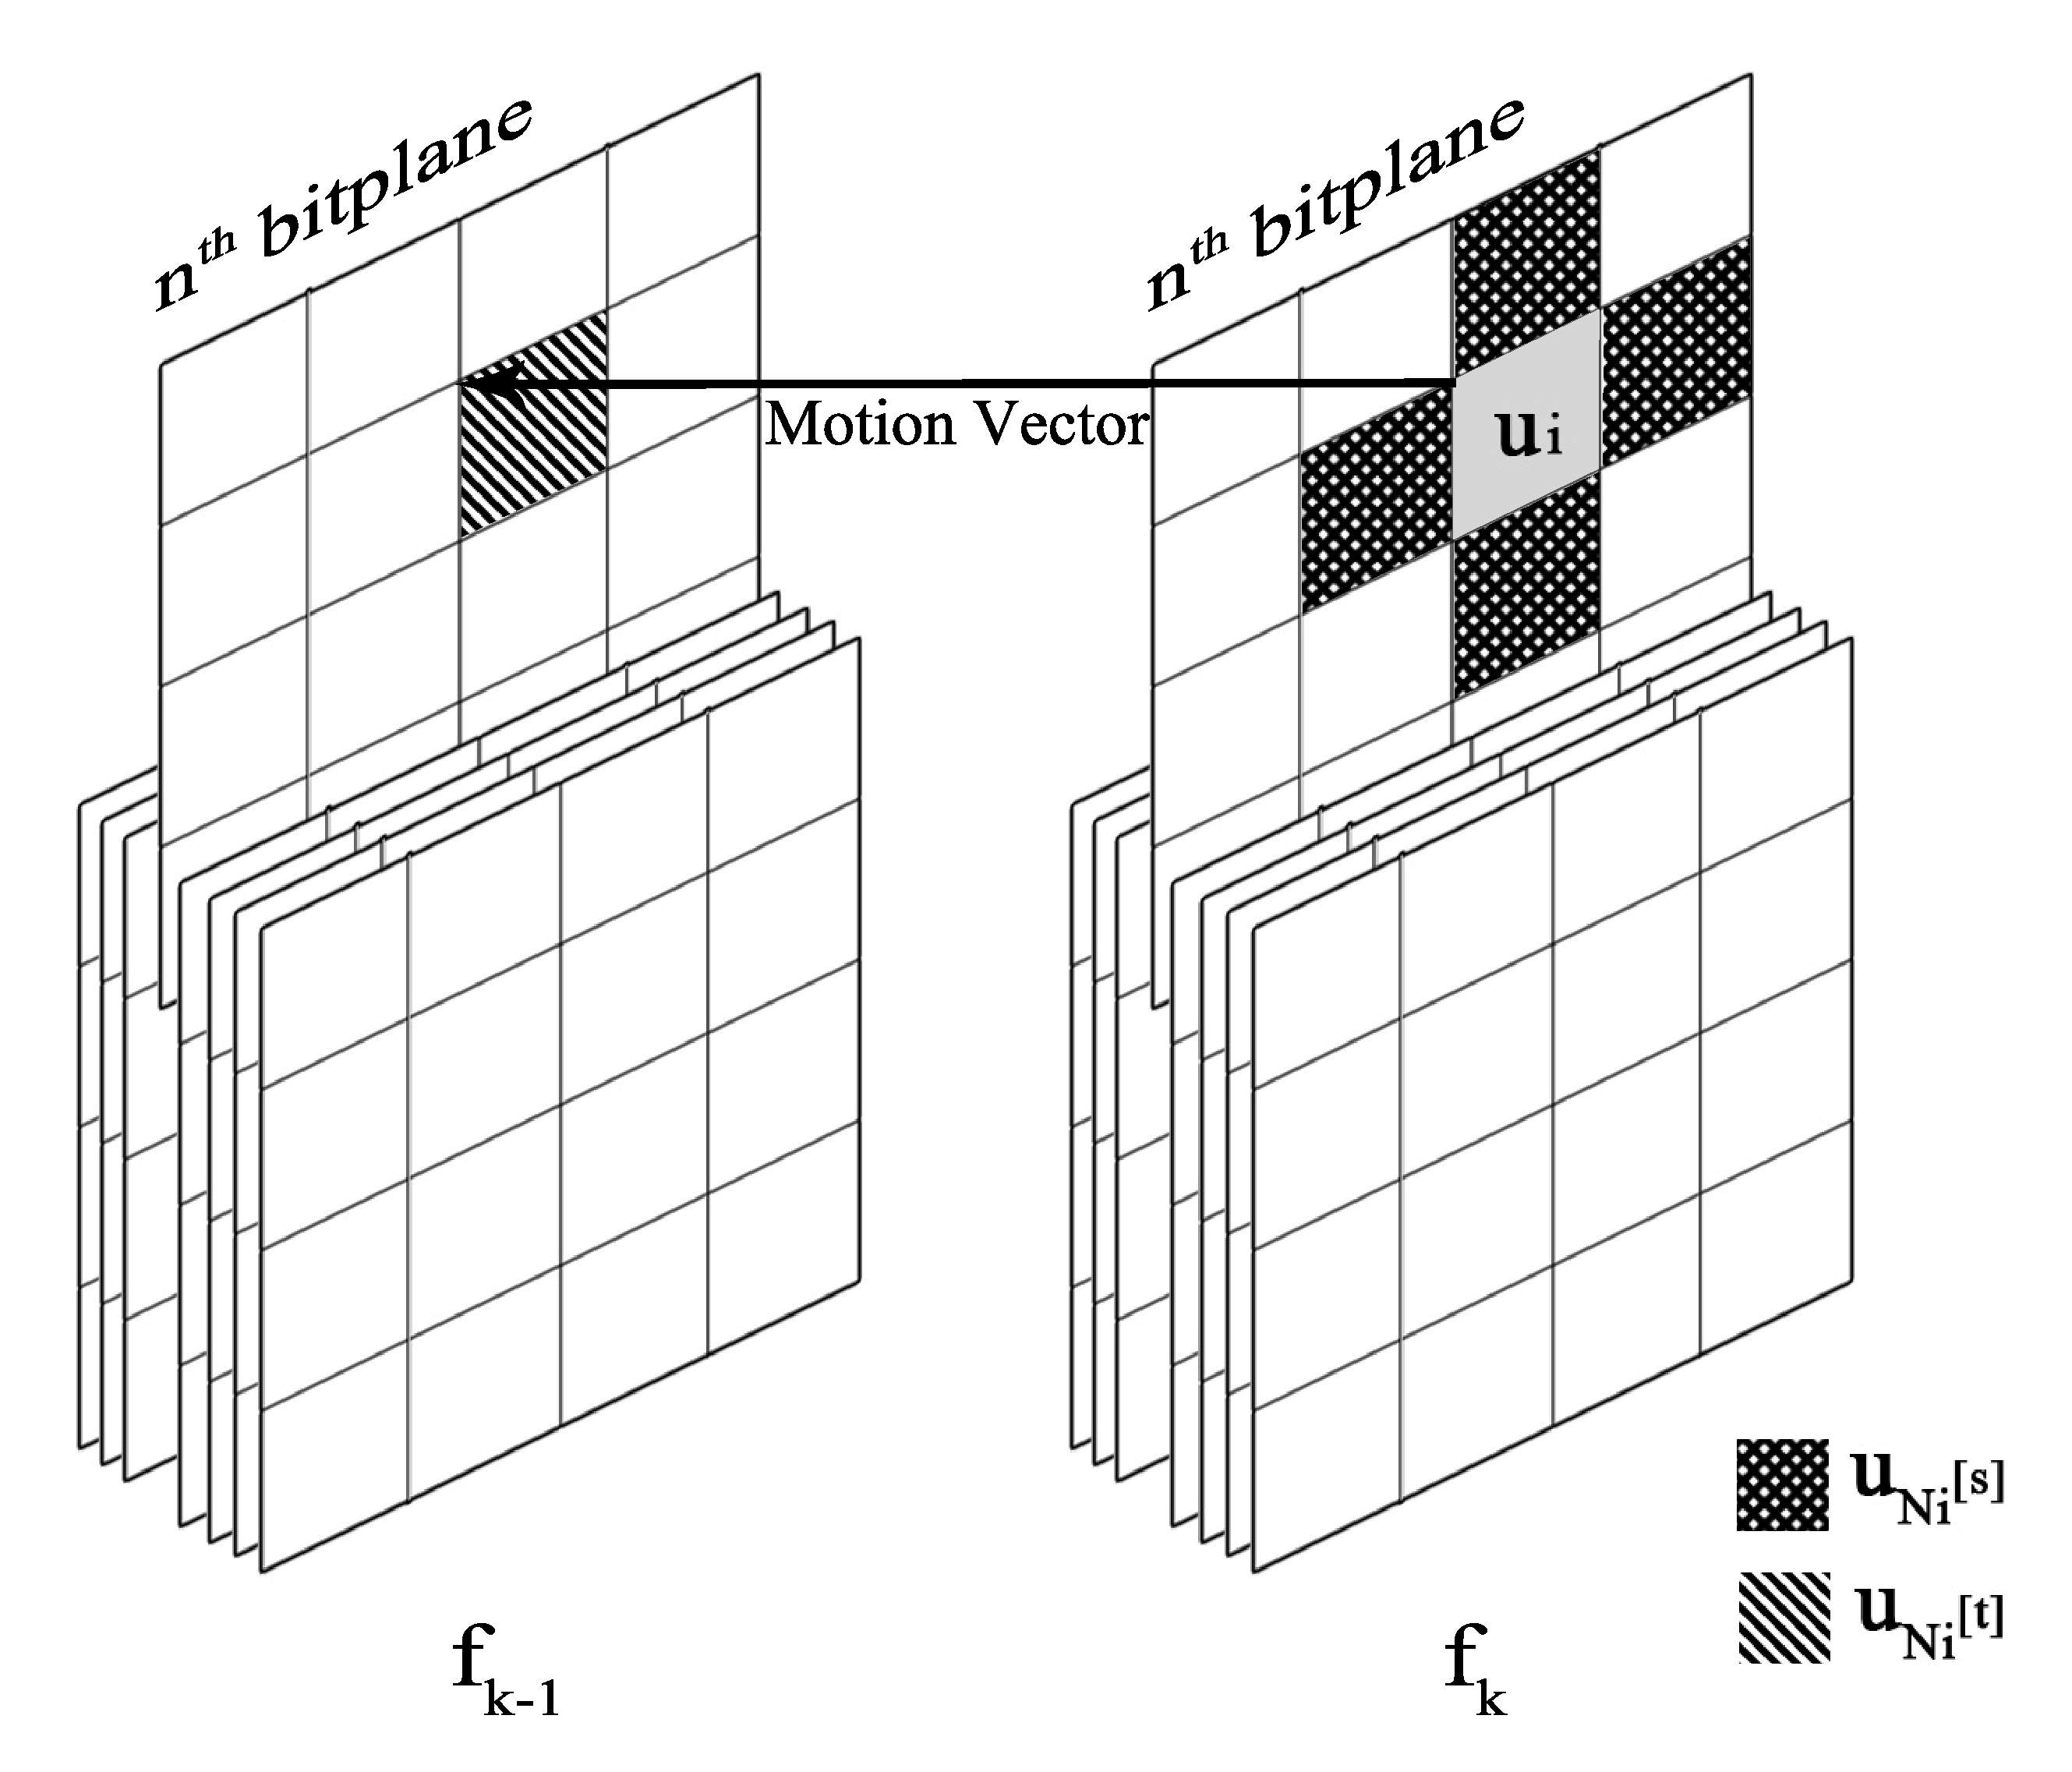
\includegraphics[height=0.25\textheight]{MRF_temporal}}
	\caption{3D-MRF model, where \ref{subfig_3DMRF_s} presents the spatial neighborhood system, and \ref{subfig_3DMRF_t} presents the temporal neighborhood system.}
\label{fig_3DMRF}
\end{figure*}

\section{3D-MRF Model}\label{sec_3dmrf}

In this section, we present the proposed three-dimensional Markov Random Field (3D-MRF) model by defining the spatial and temporal neighborhood relationship among all the bits in a transmitted video sequence and the probability of an arbitrary bit conditional on its neighborhood bits. The neighborhood relationship and the conditional probability defined by the 3D-MRF model reveals the spatial and temporal redundancy of the commonly used video sequences. Furthermore, the redundancy described by our proposed model is used to derive the 3D-MRF based soft-in soft-out source decoding, which generates the temporal and spatial extrinsic information that can be used to recover the damaged video frames.


%
%\subsection{MRF theory}
%
%The basic two elements of an MRF are sites and the labels corresponding to those sites. For example, in most image reconstruction MRF applications, a site usually refers to the position/index of a pixel, and the label is usually the corresponding pixel value in that position. For a site denoted as $i$, the corresponding label $q_i$ which takes value in $\mathcal{Q}$ is assumed to be a realization of the random variable $q_i$. Let $\mathit{S}$ be a set consisting of multiple sites with size $|\mathit{S|}$. The neighborhood system used to relate each site in $\mathit{S}$ to others is defined as
%\begin{equation}
%\mathit{N} = \{\mathit{N}_i  | \forall i \in \mathit{S}\}
%\end{equation}
%where $\mathit{N}_i$ is defined as the set consisting of an arbitrary site $i$'s neighborhood sites with respect to the neighborhood system. Furthermore, take
%\begin{equation}
%Q = \{Q_1, Q_2,...,Q_{|\mathit{S}|}\}
%\end{equation}
%as a random field consisting of all the labels of sites in $S$. A configuration $q = \{q_1,q_2,...q_{|\mathit{S}|}\} \in \mathcal{Q}^m$ is a joint realization with respect to $Q$. Given a configuration $q$, the joint event  $\{Q_1=q_1, Q_2=q_2,...,Q_{|\mathit{S}|} = q_{|\mathit{S}|}\}$ is denoted as $Q=q$, and the joint probability $P(Q=q)$ is simply represented by $P(q)$. $Q$ with the neighborhood system $\mathit{N}$ is said to be an MRF if and only if positivity and Markovianity appear in $F$. The positivity is defined by
%\begin{equation}
%P(q) > 0, \forall f \in \mathcal{Q},
%\end{equation}
%and the Markovianity says that
%\begin{equation}
%P(q_i | q_{\mathit{S} - \{i\}}) = P(q_i|f_{\mathit{N}_i}),
%\end{equation}
%where $f_{\mathit{S} - \{i\}}$ are the set of labels at all the sites in $S$ except the site $i$. The positivity as a global property implies that given an arbitrary joint realization (configuration) of $L$, there is an unique non-zero joint probability for this configuration. In other hands, Markovianity provides the local property of an MRF by saying that a site's label only depends on it's neighborhood's labels. If we specify a set of sites$\mathit{S}$, a neighborhood system $\mathit{N}$ and the conditional probability distribution $P(q_i|q_{N_i})$ of any arbitrary site's label in $\mathit{S}$, an MRF is uniquely defined.
%
%Gibbs distribution is proved to be an MRF \cite{besag1974spatial} and is widely used in MRF applications. A Gibbs distribution is defined as
%\begin{equation} \label{eq_Gibbs}
%P(q_i|q_{N_i}) = Z^{-1}\times e^{-U(q_i,q_{N_i})},
%\end{equation}
%where
%\begin{equation} \label{eq_Gibbs_Z}
%Z = \sum_{q_i \in \mathcal{Q}}e^{-U(q_i, q_{N_i})},
%\end{equation}
%and $U(q_i,q_{N_i})$ is the energy function. For a given configuration $q$ and site $i$, the energy computed by the energy function $U(q_i, q_{N_i})$ shows the local probability of the configuration $q$. When the energy value computed by $U(q_i,q_{N_i})$ is high with respect to an arbitrary site $i$ and local configuration $Q_i = q_i$, the local probability $P(q_i|q_{N_i})$ becomes low, and thus the event $Q_i = q_i$ has less chance to appear. If we only consider the first-order neighborhood relationship (i.e., the pairs of sites where each pair is constructed by a site $i$ and one of its neighborhood $i' \in \mathit{N}_i$), the energy function of a Gibbs distribution can be expanded as
%\begin{equation}
%U(q_i, q_{N_i}) = \sum_{i' \in N_i} V_{(i,i')}(q_i,q_{i'}),
%\end{equation}
%where $V_{(i,i')}(q_i,q_{i'})$ is the potential function which computes the potential between $(i, i')$, and the form of potential function $V_{(i,i')}(\cdot)$ can vary from different $(i,i')$ (e.g., geometry shape, location, ..., etc.).



\subsection{Neighborhood System of 3D-MRF Model}\label{subsec_3DMRF}

The proposed 3D-MRF model is a low-level MRF model. linking each bit of a transmitted video frame to it's surrounding bits both in spatial and temporal direction as depicted in {Fig. \ref{fig_3DMRF}}. For simplicity, a single bit $u_{k,n}^{(x,y)}$ mentioned in Section \ref{sec_sm} is denoted as $u_i$, where a single index $i$ comprises the indices $(k,n,x,y)$. In the 3D-MRF model, we aim to describe the redundancy in a video sequence by defining the neighborhood bits of each bit in the decoding video sequence. The neighborhood bits of an arbitrary bit denoted by $u_i$ are supposed to be similar to the bit $u_i$, and those neighborhood bits can therefore help the decoding of the bit $u_i$ by providing the extrinsic information. The set consisting of the neighborhood bits of the arbitrary bit $u_i$ is denoted by $\mathit{N}_i $, and $\mathit{N}_i $ can be separated into two subsets as
\begin{equation}
\mathit{N}_i = N_i^{[s]} \cup N_i^{[t]}, 
\end{equation}
where $N_i^{[s]}$ is the spatial neighborhood subset consisting of the spatial neighborhood bits of $u_i$. Likewise, the subset $N_i^{[t]}$ is the temporal neighborhood subset which comprises the temporal neighborhood bits of $u_i$. We separate the neighborhood bits of $u_i$ into two subsets in order to control the extrinsic information provided by the spatial neighborhood bits and the temporal neighborhood bits.

Regarding the spatial homogeneity, we choose $4$ nearest bits in the same bit-plane with $u_i$ to form the spatial two dimensional neighborhood system as illustrated in Fig. \ref{fig_3DMRF}. Thus, the spatial subset $N_i^{[s]}$ is defined as
\begin{equation}
u_{N_i^{[s]}} = \{ u_{k,n}^{(x-1,y)}, u_{k,n}^{(x+1,y)}, u_{k,n}^{(x,y-1)}, u_{k,n}^{(x,y+1)} \}.
\label{eq_Nis}
\end{equation}

Furthermore, considering the temporal subset $N_i^{[t]}$, we propose using the decoder-side motion estimation to locate the local motion vectors between received video frames, which will be detailed in Section \ref{sec_alg}. Through the local motion vector, a pixel $f_{k}^{(x,y)}$ at location $(x,y)$ in frame $k$ is related to another pixel $f_{k-1}^{(x',y')}$ at location $(x',y')$ in the previous frame $k-1$, where $(x',y')$ is computed from decoder side motion estimation. As a result, we let those bits in $\mathbf{f}_{k-1}$ which is located by the motion vector becomes the temporal neighborhood sites of bits in $\mathbf{f}_{k}$ to show the temporal redundancy in the MRF model, and thus the temporal neighborhood subset is
\begin{equation}
u_{N_i^{[t]}} = \{u_{k-1,n}^{(x',y')}, x' = x - v_i^x, y' = y - v_i^y\},
\label{eq_Nit}
\end{equation} 
where $(v_i^x,  v_i^y)$ is the local motion vector which belongs to $u_i$. 

The reason why we choose the basic element in 3D-MRF to be represented by a single bit in a bit-plane of a video frame instead of the pixel value from the $m$-bit pattern is mainly due to the complexity issue.  The decoding process chosen by soft decoding is either a maximum likelihood (ML) or maximum \textit{a posteriori} probability (MAP) decision, where both require a number of $2^m$ probability computation if a $m$-bit pattern is assumed to be decoded. By using our proposed bit-plane level MRF model, the decoding process is simplified from single decision problem with complexity $O(2^m)$ to $m$ decision problems, where each one is a $0/1$ decision problem and the total complexity is $O(2m)$. Taking $m=8$ as a common set-up, the decoding complexity of a pixel is $16$ times lower than the conventional one, resulting a significant complexity improvement.

\subsection{Conditional Probability of 3D-MRF Model}

The probability of an arbitrary bit $u_i$ conditional on its neighborhood bits in 3D-MRF takes the form
\begin{equation}
P(u_i | u_{N_i}) = Z^{-1}\times e^{-U(u_i,u_{N_i})}.
\label{eq_3DMRF_prob}
\end{equation}
The conditional probability form in \ref{eq_3DMRF_prob} is Gibbs distribution \cite{besag1974spatial}, which is widely used in MRF applications. The $Z$ is simply a normalization terms defined by
\begin{align}
Z =& \sum_{u_i \in \{0,1\}}e^{-U(u_i, u_{N_i})}\\
=& e^{-U(u_i=0, u_{N_i})} + e^{-U(u_i=1, u_{N_i})}.
\end{align}
The energy function $U(u_i,u_{N_i})$ describes the potential energy between $u_i$ and the neighborhood bits $u_{N_i}$. When the potential energy is higher, the conditional probability of $u_i$ conditional on $u_{N_i}$ becomes lower as shown in (\ref{eq_3DMRF_prob}), and vise versa. We define the energy function $U(u_i,u_{N_i})$ by the summation of both spatial and temporal neighborhood pairs' potential as
\begin{equation}
U(u_i, u_{N_i}) =  \sum_{i'  \in N_i^{[s]}}V_c^{[s]}(u_i, u_{i'}) + \sum_{i'  \in N_i^{[t]}} V_c^{[t]}(u_i, u_{i'}).
\label{eq_energy_function}
\end{equation}
By assuming each bit-plane is a piecewise constant surface, we let the potential functions $V_c^{[s]}$ and $V_c^{[t]}$ take the form
\begin{equation}
V_c^{[s]}(u_i, u_{i'}) = \beta_s (1- \delta(u_i - u_{i'}))
\label{eq_potential_spatial}
\end{equation}
and
\begin{equation}
V_c^{[t]}(u_i, u_{i'}) = \beta_t (1- \delta(u_i - u_{i'})),
\label{eq_potential_temporal}
\end{equation}
where $\delta(u)$ is the Dirac delta function, and $\delta(u) = 1$ only when $u=0$. In other words, for each neighborhood pair $(u_i, u_{i'}),\ i' \in N_i$, if $u_i \neq u_{i'}$, a penalty term is added to the energy function $U(u_i, u_{N_i})$, where the penalty term is $\beta_s$ or $\beta_t$ according to whether $u_{i'}$ is a spatial neighborhood site or a temporal one. The penalty coefficient $\beta_s$ and $\beta_t$ represent the homogeneity of the transmitted video sequence, where a high value of a penalty coefficient implies that there is a significant similarity between the neighborhood sites in 3D-MRF. In our proposed decoding method, $\beta_s$ and $\beta_t$ are estimated from the video content on-the-fly for each frame and bit-plane. 

\subsection{3D-MRF Based SISO Source Decoding}\label{subsec_3DMRF_SISO}
The source decoder based on proposed 3D-MRF model is an SISO decoder, where the inputs and outputs are both LLRs of each bit in the transmitted video sequences. For a single bit $u_i$, the input {\it a priori} LLR of $u_i$ is denoted as
\begin{equation}
L_i^{(I)} = L_s^{(I)}(u_i) = \ln \frac{P(u_i = 0)}{P(u_i = 1)}.
\end{equation}
We derive the decoding method through the {\it a posteriori} probability based on proposed 3D-MRF model. For each bit, the {\it a posteriori} probability output can be represented by the {\it a posteriori} LLR
\begin{equation}
L_i^{(O)} =\ln \frac{P(u_i = 0 | L^{(I)}_i, L^{(I)}_{N_i})}{P(u_i = 1 | L^{(I)}_i, L^{(I)}_{N_i})},
\label{eq_LLR_app}
\end{equation}
where $L_{N_i}^{(I)}$ is the set composed of input {\it a priori} LLRs of $N_i$ which is the neighborhood of $u_i$ in proposed 3D-MRF model. From Bayes' theorem and the fact that $P(u_i) = 1/2$ and $\ln(P(u_i=0)/P(u_i  =1)) = 0$ when the probability is not conditional on the input {\it a priori} information $L^{(I)}_i$, (\ref{eq_LLR_app}) can be modified as
\begin{align}
L_i^{(O)} &= \ln \frac{P(u_i = 0, L^{(I)}_i, L^{(I)}_{N_i})}{P(u_i = 1, L^{(I)}_i, L^{(I)}_{N_i})}\nonumber  \\
&= \ln \frac{P(L^{(I)}_i | u_i = 0,  L^{(I)}_{N_i})}{P(L^{(I)}_i | u_i = 1,  L^{(I)}_{N_i})} + \ln \frac{P(u_i = 0 | L^{(I)}_{N_i})}{P(u_i = 1 | L^{(I)}_{N_i})}.
\label{eq_LLR_app_bayes}
\end{align}
Also, since that $L^{(I)}_i$ and $L^{(I)}_{N_i}$ are conditionally independent when $u_i$ is given, (\ref{eq_LLR_app_bayes}) is further derived as
\begin{equation}
L_i^{(O)} = \ln \frac{P(u_i = 0| L^{(I)}_i)}{P(u_i = 1|L^{(I)}_i)} + \ln \frac{P(u_i = 0| L^{(I)}_{N_i})}{P(u_i = 1|L^{(I)}_{N_i})},
\end{equation}
where the first term are simply $L_i^{(I)}$ itself, and the second term is the probabilities conditional on $N_i$ described from the 3D-MRF model. However, for each bit in $N_i$, we have only their LLRs instead of the exact value of $u_{N_i}$, and thus the conditional probability in (\ref{eq_3DMRF_prob}) of 3D-MRF model cannot be directly used in the derivation. In conventional MAP-MRF decoding method, this problem is usually solved by a iterative process, where in each iteration the $\hat{u}_{N_i}$ estimated from $L_{N_i}$ is used to derive the conditional probability of $u_i$, and thus imposes computation complexity. We propose a novel solution which can exploit the uncertainty of $N_i$ with a low computation overhead at the same time. We modify the conditional probability of $u_i$ based on the expectation of the energy function $U(u_i, u_{N_i})$ over $L_{N_i}$ as
\begin{align}
P(u_i|L_{N_i}) &= Z^{-1}\times e^{-E[U(u_i, u_{N_i})| L_{N_i}]},
\label{eq_app_exp}
\end{align}
where $E[\cdot]$ is the expectation function based on a given probability distribution. From (\ref{eq_energy_function}), the expectation of energy function is 
\begin{align}
E[U(u_i, u_{N_i})| L_{N_i}] &=  \sum_{i'  \in N_i^{[s]}}E[V_c^{[s]}(u_i, u_{i'})|L_{i'}] \nonumber \\
&+ \sum_{i'  \in N_i^{[t]}} E[V_c^{[t]}(u_i, u_{i'})|L_{i'}],
\label{eq_energy_function_exp}
\end{align}
Furthermore, the potential functions in (\ref{eq_energy_function_exp}) can be simplified by taking expectation on each neighborhood pair's potential in (\ref{eq_potential_spatial}) and (\ref{eq_potential_temporal}) over the LLR values as
\begin{equation}
E[V_c^{[s]}(u_i, u_{i'})|L_{i'}] = \beta_s (P(u_{i'} \neq u_i | L_{i'}))
\label{eq_potential_spatial_exp}
\end{equation}
and
\begin{equation}
E[V_c^{[t]}(u_i, u_{i'})|L_{i'}] = \beta_t (P(u_{i'} \neq u_i | L_{i'})),
\label{eq_potential_temporal_exp},
\end{equation}
where $\beta_s$ and $\beta_t$ are the 3D-MRF parameter of the decoding video.
By combining (\ref{eq_LLR_app})-(\ref{eq_potential_temporal_exp}), the {\it a posteriori} LLR in (\ref{eq_LLR_app}) can be shown as
\begin{IEEEeqnarray}{rCl}
L_i^{(O)} & =  &\ln \frac{P(u_i = 0|L_{N_i}) }{P(u_i = 1|L_{N_i}) } + \ln \frac{P(u_i = 0|L_i)}{P(u_i = 1|L_i)} \\
& = &\sum_{i'  \in N_i^{[s]}} \beta_s (P(u_{i'} = 1 | L_{i'}) - P(u_{i'} = 0 | L_{i'}))  \nonumber \\
&& + \sum_{i'  \in N_i^{[t]}} \beta_t(P(u_{i'} = 1 | L_{i'}) - P(u_{i'} = 0 | L_{i'})) \nonumber \\
&& + L_i,
\label{eq_app_LLR_final}
\end{IEEEeqnarray}
where the first term and second term correspond to the extrinsic information of spatial part and temporal part in 3D-MRF respectively, and the third term is simply the {\it a priori} information. Thus, we reformulate the 3D-MRF decoding output as
\begin{equation}
L_i^{(O)} = L_i^{(E,s)} + L_i^{(E,t)} + L_i^{(I)},
\end{equation} 
where $L_i^{(E,s)}$ and $L_i^{(E,t)}$ are the first term and second term in (\ref{eq_app_LLR_final}). It shows that we can separately compute the extrinsic information $L_i^{(E,s)}$ and $L_i^{(E,t)}$ solely from the LLR of $u_i$'s neighborhood without $L_i$ involved, which is convenient for the iterative source-channel decoding discussed in Section \ref{sec_alg}.


\begin{figure*}[t]
\centering
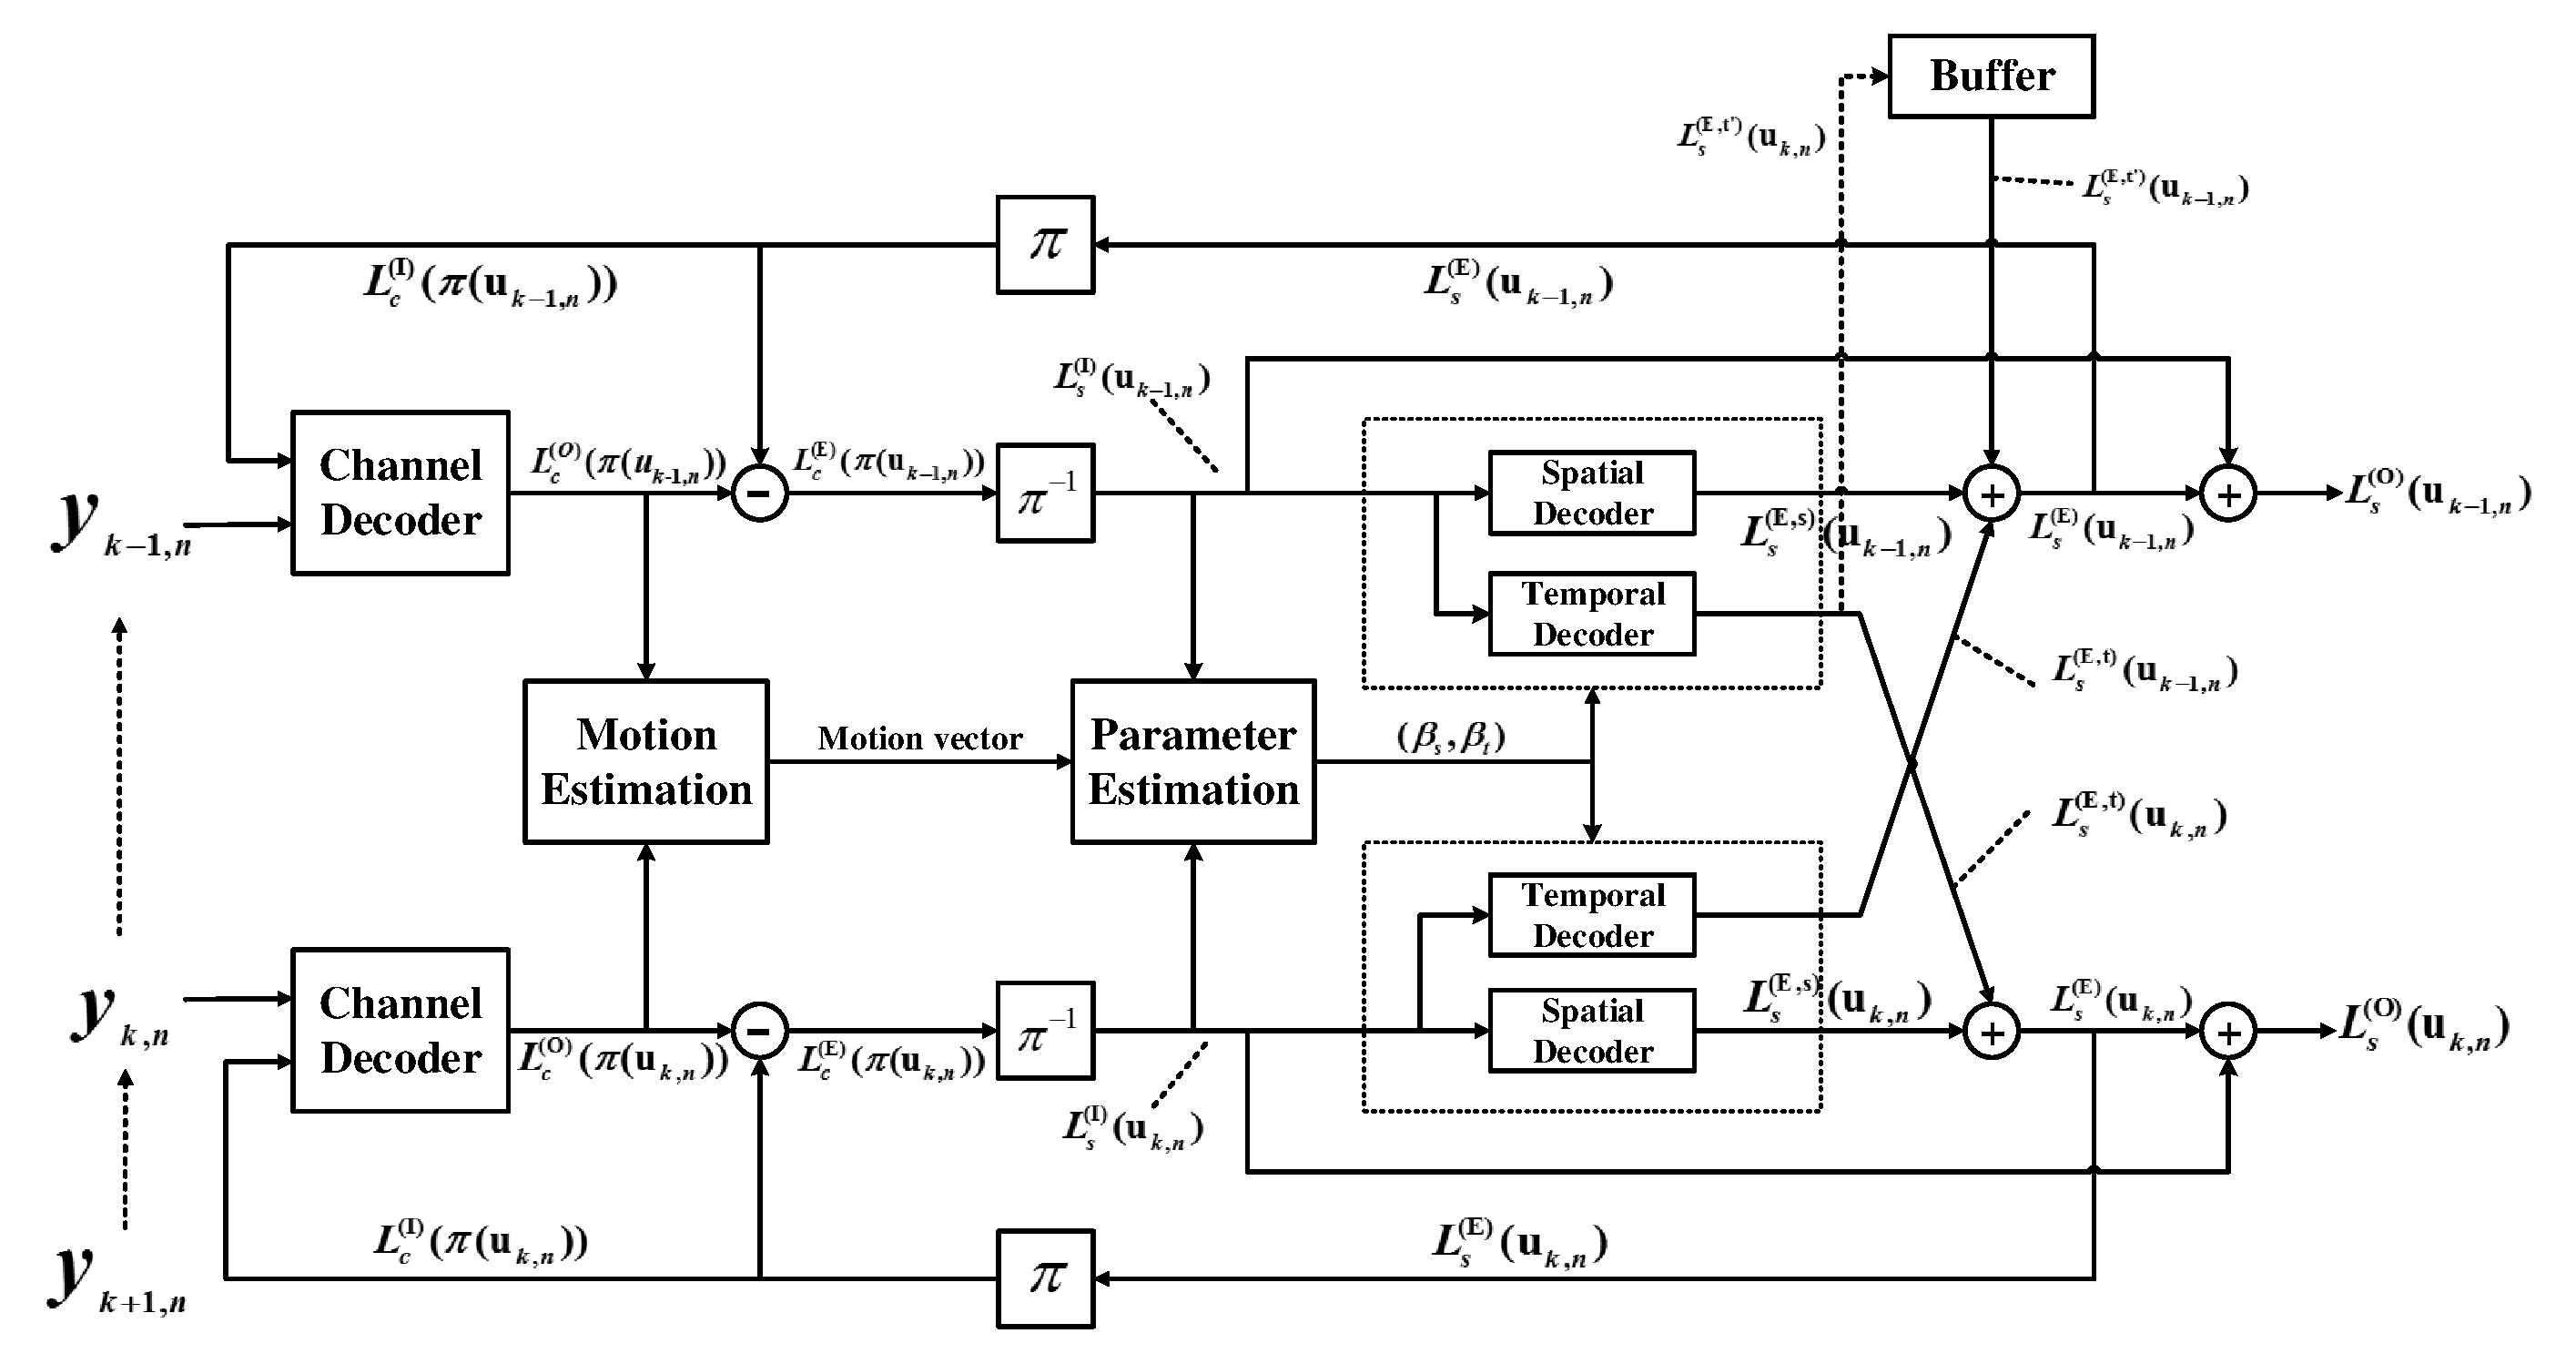
\includegraphics[width=\textwidth]{block_diagram_test.pdf}
\caption{3D-MRF based Iterative source-channel decoder structure.}
\label{cf_de}
\end{figure*}

\section{Iterative Channel-Source Decoding Algorithm}\label{sec_alg}

In this section, the iterative channel-source decoding algorithm based on the proposed 3D-MRF is presented. The iterative decoder structure is shown in Fig. \ref{cf_de}, where the iterative decoding of two consecutive received frames is performed by the extrinsic information exchange between channel decoder and source decoder, as well as between two consecutive received video frames. In the following subsections, we firstly introduce the decoder side motion estimation, which is used to locate the temporal neighborhood. Then the 3D-MRF parameter estimation is derived using a least square error solution. Along with the 3D-MRF based SISO source decoding proposed in \ref{subsec_3DMRF_SISO}, the iterative decoding flow is finally detailed in \ref{subsec_iter_process}.

\subsection{Decoder Side Motion Estimation}
%Recently, distributed video coding (DVC) has become a popular research topic in video compression/transmission domain since it claims that it could achieve the same rate-distortion performance as conventional video codec while the computational load is shifted to the decoder side \cite{DVC}. Winer-Ziv codec, based on the Wyner-Ziv theorem \cite{Wyner_ziv}, is the state-of-art implementation structure of DVC\cite{Wyner_ziv_coding}. In Wyner-Ziv codec, the decoder side motion estimation is used to generate the side information of a Winer-Ziv frame, which is a interpolation of received intra-coded frame. However,

In the proposed 3D-MRF model, the temporal neighborhood system aims to describe the temporal redundancy of the commonly used video sequences. Though the nearby video frames usually have high similarity, the movement of pixels should not be ignored. In the conventional video compression, motion estimation is the widely-used tool to locate the movement between the video frames, and thus the temporal redundancy can be removed in the video compression process. Also, in the distributed video coding (DVC) \cite{DVC}, the motion estimation is implemented in the decoder side to generate the side information of a Winer-Ziv frame \cite{Wyner_ziv_coding}, which is an interpolation of received intra-coded frame. Therefore, we select the decoder side motion estimation as the tool to describe the temporal redundancy. 

However, different from the conventional video compression and DVC, in our work, the decoder side motion estimation is used to locate the temporal neighborhood relationships in proposed 3D-MRF model mentioned in \ref{subsec_3DMRF} between received uncompressed video frames. In our decoder side motion estimation, a received and decoded video frame $\hat{\mathbf{f}}_{k}$ is divided into several macro-blocks (MB), each of whom consists of several pixels in $\hat{\mathbf{f}}_{k}$. For an $i$-th MB in $\hat{\mathbf{f}}_{k}$ denoted as $\mathbf{b}_{k,i}$, it searches for a motion vector $v_{k,i} = (v_{k,i}^x, v_{k,i}^y)$ such that
\begin{equation}
v_{k,i} = \argmin_{v_{k,i}^x, v_{k,i}^y \in \{-d,d\}} \sum_{\hat{f}_k^{(x,y)} \in \mathbf{b}_{k,i}} c(\hat{f}_k^{(x,y)}, \hat{f}_{k-1}^{(x- v_{k,i}^x, y - v_{k,i}^y)}),
\label{eq_ME}
\end{equation}
where $d$ is the search range, and $c(f,f')$ is the cost function between two pixels $f$ and $f'$. We use mean absolute deviation (MAD) as the cost function, where
\begin{equation}
c(f,f') = |f-f'|,
\end{equation}
where $|\cdot|$ is the absolute value.
As a result, for each pixel $\hat{f}_k^{x,y} \in \mathbf{b}_{k,i}$, there is a corresponding pixel in the previous frame $\hat{\mathbf{f}}_{k-1}$ indicated by the motion vector $v_{k,i}$. After acquiring the local motion vector for a pixel $\hat{f}_k^{x,y}$, the temporal neighborhood bit $N_{i}^{[t]}$ of a bit $\hat{u}_{k,n}^{(x,y)}$ is located through (\ref{eq_Nit}) with the motion vector $v_{k,i}$. It is worth noting that the same motion vector $v_{k,i}$ located by $\hat{f}_k^{x,y}$ is used for every bit of the single pixel.

\subsection{Parameter Estimation}\label{subsec_par_est}
In this subsection, the parameter estimation of $\beta_s$ and $\beta_t$, as ``Parameter Estimator" illustrated in Fig. \ref{cf_de}, is performed by the least-square fit solution first proposed by \cite{Gibbs_par}. Consider the conditional probability $P(u_i|u_{N_i})$ in (\ref{eq_3DMRF_prob}) where the left-hand side is modified by Bayes' theorem as
\begin{equation}
\frac{P(u_i, u_{N_i})}{P(u_{N_i})} = \frac{e^{-U(u_i,u_{N_i})}}{e^{-U(0, u_{N_i})} + e^{-U(1, u_{N_i})}}.
\end{equation}
Rearranging the above equation, we yield
\begin{equation}
\frac{e^{-U(0, u_{N_i})} + e^{-U(1, u_{N_i})}}{P(u_{N_i})} = \frac{e^{-U(u_i,u_{N_i})}}{P(u_i, u_{N_i})}.
\label{eq_3DMRF_prob_rearrrange}
\end{equation}
Note that the left-hand side in (\ref{eq_3DMRF_prob_rearrrange}) is independent to whether $u_i$ is $0$ or $1$. Therefore, substitute $u_i=0$ and $u_i = 1$ into the right-hand side of (\ref{eq_3DMRF_prob_rearrrange}) and link them through the left-hand side of (\ref{eq_3DMRF_prob_rearrrange}), we have
\begin{equation}
\frac{e^{-U(u_i = 0,u_{N_i})}}{P(u_i = 0, u_{N_i})} = \frac{e^{-U(u_i = 1,u_{N_i})}}{P(u_i = 1, u_{N_i})}.
\label{eq_PS_01}
\end{equation}
Again we rearrange and take the logarithm of two sides in (\ref{eq_PS_01}) as
\begin{equation}
\ln(\frac{e^{-U(u_i = 0,u_{N_i})}}{e^{-U(u_i = 1,u_{N_i})}}) = \ln(\frac{P(u_i = 0, u_{N_i})}{P(u_i = 1, u_{N_i})}).
\label{eq_PS_log_01}
\end{equation}
Substitute (\ref{eq_potential_spatial}) and (\ref{eq_potential_temporal}) into the left-hand side of (\ref{eq_PS_log_01}), and we have
\begin{equation}
\beta_s x_i^{[s]} + \beta_t x_i^{[t]} = y_i,
\label{eq_PS_Linear}
\end{equation}
where
\begin{align}
x_i^{[s]} &= \#\{u_{N_i^{[s]}} = 0\} - \#\{u_{N_i^{[s]}} = 1\},\\
x_i^{[t]} &= \#\{u_{N_i^{[t]}} = 0\} - \#\{u_{N_i^{[t]}} = 1\}, \\
\end{align}
and
\begin{align}
y_i &=  \ln(\frac{P(u_i = 0, u_{N_i})}{P(u_i = 1, u_{N_i})}).
\end{align}
Note that (\ref{eq_PS_Linear}) is a linear equation with respect to $\beta_s$ and $\beta_t$, which implies that $\beta_s$ and $\beta_t$ can be obtained from linear equations once we have  $P(u_i,u_{N_i})$. This problem is solved by histogram technique. Assume we have a sample set $\mathbf{u}$ consisting of multiple bits in 3D-MRF with size $|\mathbf{u}|$. Using histogram technique, the local joint probability can be expressed as
\begin{equation}
P(u_i, u_{N_i}) = \frac{H(u_i, u_{N_i})}{|\mathbf{u}|},
\end{equation}
where $H(u_i, u_{N_i})$ is the histogram count of the local configuration $(u_i, u_{N_i})$ occurs in $\mathbf{u}$, and therefore
\begin{equation}
y_i =  \ln(\frac{H(u_i = 0, u_{N_i})}{H(u_i = 1, u_{N_i})}).
\end{equation}

To obtain $\beta_s$ and $\beta_t$ from the sample set $\mathbf{u}$, we denote $x_i^{[s]}$ and $x_i^{[t]}$ of the sample set $\mathbf{u}$ as two column vectors. Using the linear equation in (\ref{eq_PS_Linear}), we obtain the simultaneous linear equations  
\begin{equation}
\begin{pmatrix}
x_1^{[s]} & x_1^{[t]} \\
x_2^{[s]} & x_2^{[t]} \\
\vdots & \vdots \\
x_{|\mathbf{u}|}^{[s]} & x_{|\mathbf{u}|}^{[t]} \\
\end{pmatrix}
\begin{pmatrix}
\beta_s \\
\beta_t
\end{pmatrix}
=
\begin{pmatrix}
y_1 \\
y_2 \\
\vdots \\
y_{|\mathbf{u}|}
\end{pmatrix},
\end{equation}
which is an overdetermined system simply denoted as
\begin{equation}
\mathbf{X}
\begin{pmatrix}
\beta_s \\
\beta_t
\end{pmatrix}
 = \mathbf{Y}.
\end{equation}
Thus, $\beta_s$ and $\beta_t$ can be estimated with a conventional least-square solution :
\begin{equation}
\begin{pmatrix}
\beta_s \\
\beta_t
\end{pmatrix}
= \mathbf{X}^{\dagger}\mathbf{Y},
\label{eq_beta_est}
\end{equation}
where $\mathbf{X}^{\dagger}$ is the Moore-Penrose pseudoinverse of matrix $\mathbf{X}$. It is worth noting that the parameter estimation mentioned here is performed with each bit-plane separately. 

\subsection{Iterative Process}\label{subsec_iter_process}
With the estimator and the extrinsic information equation, the iterative decoding process is performed with the following steps as shown in Fig. \ref{cf_de}:
\begin{enumerate}
\item \label{s1} Initialize the {\it a prior} information of two SISO channel decoder by setting all bits to be equiprobable (i.e., set $L_c^{(I)}$ to be all zero.)

\item \label{s2} For each frame, pass the received signals $\mathbf{y}$ with {\it a priori} information $L_c^{(I)}$ through the SISO channel decoders, and get the output LLR values $L_c^{(O)}$. The extrinsic information LLRs $L_c^{(E)}$ are computed through subtracting the {\it a priori} LLRs $L_c^{(I)}$ from the output LLRs $L_c^{(O)}$.

\item \label{s3} Compute the local motion vector from the channel decoded and deinterleaved two consecutive frames $\hat{\mathbf{f}_k}$ and $\hat{\mathbf{f}_{k-1}}$ using (\ref{eq_ME}), and locate the temporal neighborhood of each bit using (\ref{eq_Nit}).

\item \label{s4} Estimate the 3D-MRF parameter $\beta_s$ and $\beta_t$ for each bit-plane using (\ref{eq_beta_est}) mentioned in Section \ref{subsec_par_est}.

\item \label{s5} Pass the deinterleaved channel output extrinsic LLRs as the input {\it a priori} LLRs $L_s^{(I)}$ to the 3D-MRF based SISO source decoder based on the 3D-MRF parameter estimated in step \ref{s4}. In the source decoder, use (\ref{eq_app_LLR_final}) to obtain the spatial and temporal extrinsic information, denoted as $L_s^{(E,s)}$ and $L_s^{(E,t)}$, respectively.

\item \label{s6} Obtain the joint source extrinsic LLRs $L_s^{(E)}$ of frame $k-1$. Sum up the spatial extrinsic information $L_s^{(E,s)}$, the temporal extrinsic information $L_s^{(E,t)}$, and the buffered temporal extrinsic information $L_s^{(E,t')}$ of previous decoding cycle, which is actually the temporal information from frame $k-2$.

\item \label{s6'} Obtain the joint source extrinsic LLRs $L_s^{(E)}$ of frame $k$ by summing up the spatial extrinsic information $L_s^{(E,s)}$ and the temporal extrinsic information $L_s^{(E,t)}$. Buffer the temporal extrinsic information $L_s^{(E,t)}$ as $L_s^{(E,t')}$ if it is the last iteration.

\item \label{s7} Pass the extrinsic information of source decoder $L_s^{(E)}$ through the interleavers to acquire the {\it a prior} information $L_c^{(I)}$ for channel decoder, which is used for the next iteration.

\item If not the final iteration, go to step \ref{s2}. Otherwise, pass the output LLR values of all bit planes, which is the summation of $L_s^{(I)}$ and $L_s^{(E)}$, denoted as $L^{(O)}$,  through a simple sign detector and combine them to form the decoded frames.
\end{enumerate}

\begin{figure*}[!t]
	\centering
	\subfloat[]{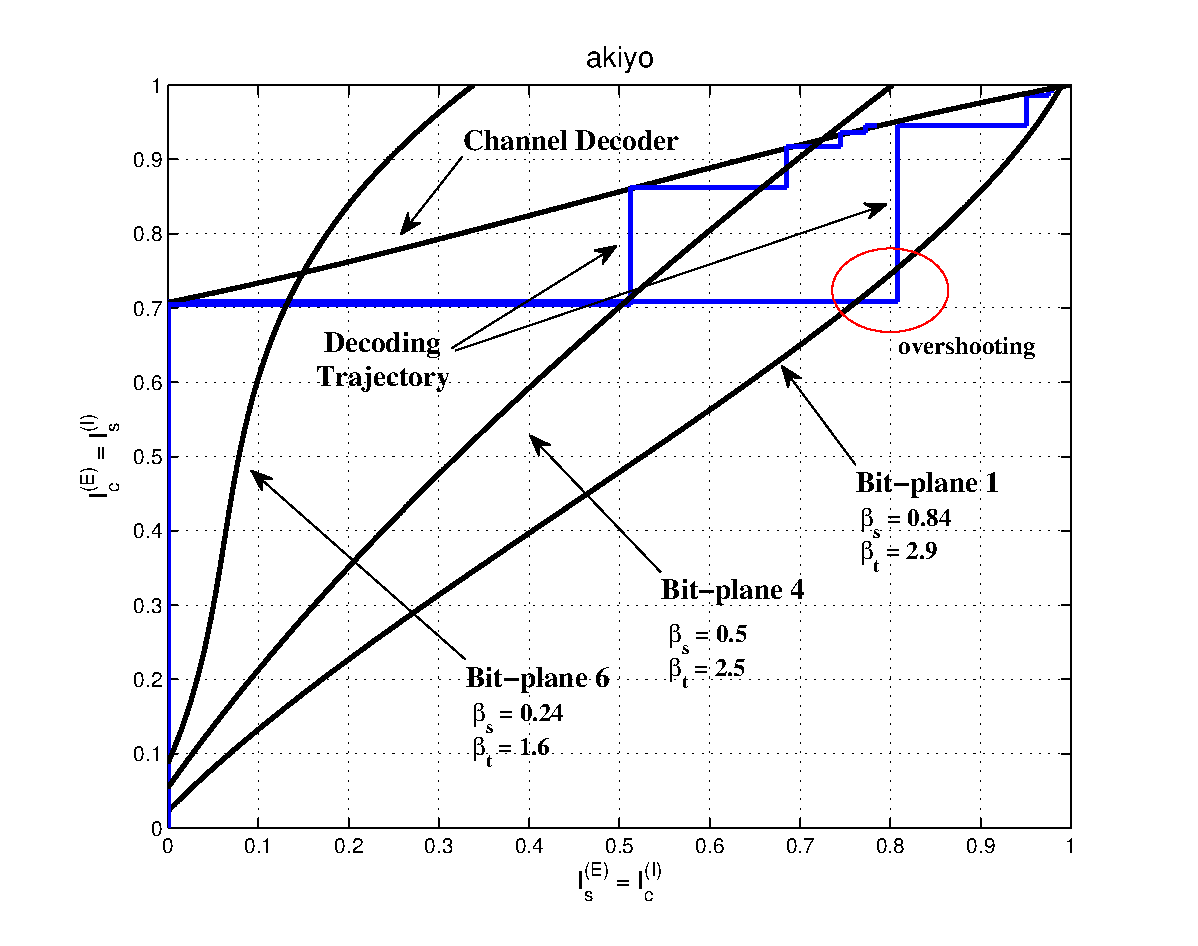
\includegraphics[width=0.5\textwidth]{akiyo_f3_bp146}}
	\subfloat[]{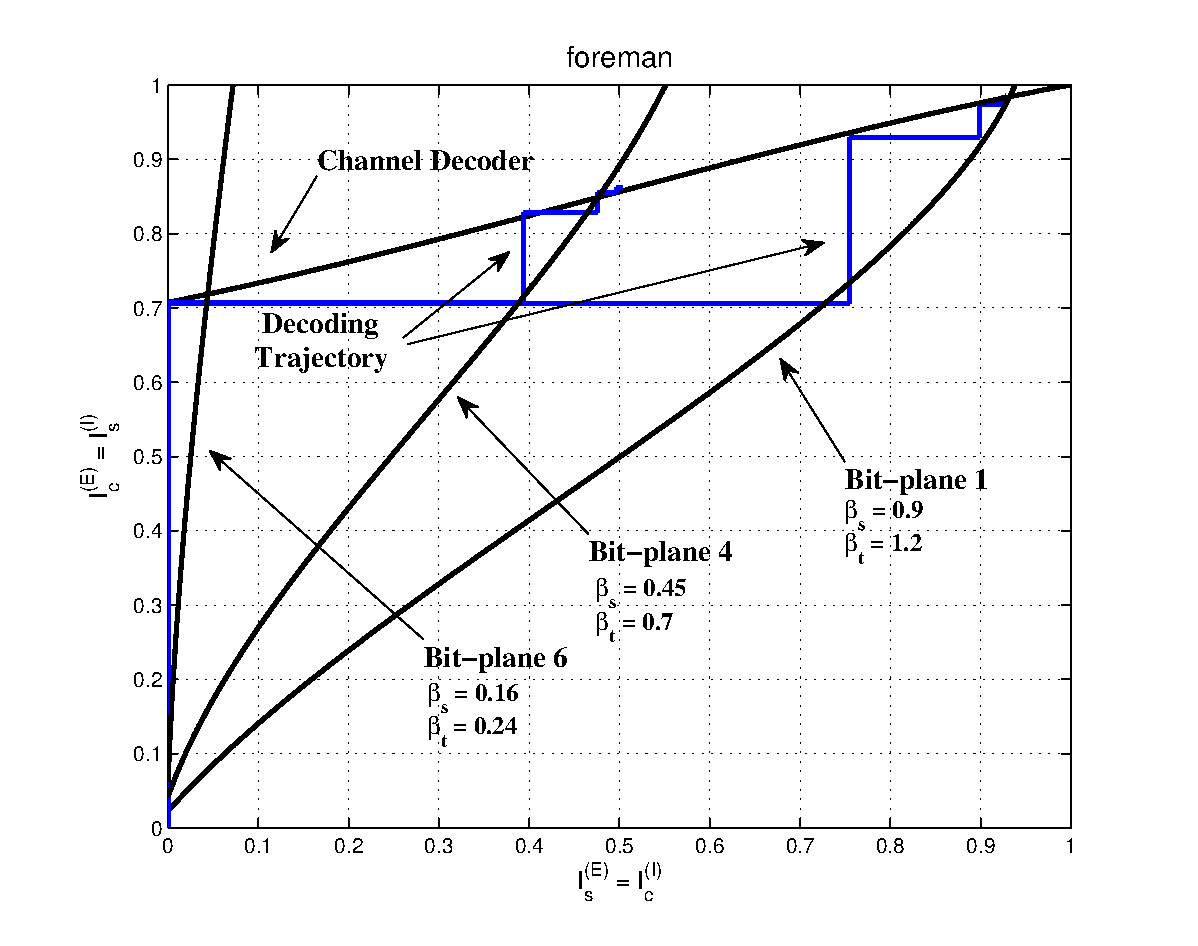
\includegraphics[width=0.5\textwidth]{foreman_f3_bp146}}
	\caption{EXIT charts of proposed ISCD method using the ``akiyo" and the ``foreman" sequences with SNR equals $0$.}
	\label{fig_exit}
\end{figure*}

The iterative decoder design follows few basic ideas. First, to avoid the overlapping information, only the extrinsic information is exchanged between channel and source decoders. Second, since the goal of the decoder side motion estimation is to locate the temporal neighborhood bits in 3D-MRF, it is naturally to use the full {\it a posteriori} information instead of the extrinsic information as the input of motion estimation. Third, the temporal information can be both obtained from the previous and the next frame. However, the complexity and latency would dramatically increase if we decoding $3$ frames simultaneously. Therefore, we design a consecutive decoding process to keep the temporal extrinsic information propagating from frame to frame without the increase of complexity and latency. We put a buffer in the decoder structure to buffer the temporal extrinsic information (step \ref{s6'}) from the previous frame, and thus it could be used (step \ref{s6}) to improve the source decoding when the next video frame is received.

The iterative source-channel decoder shown in Fig. \ref{cf_de} have the properties of both serial concatenated codes (SCCC) and parallel concatenated codes (PCCC). In the serial direction, the 3D-MRF spatial redundancy can be seen as an outer code in SCCC, and the channel code, which encodes the video frames generated by the 3D-MRF redundancy, is seen as the inner code in SCCC. Thus, the extrinsic information exchanging process between the 3D-MRF based spatial decoder and the channel decoder in the proposed ISCD process presents the serial concatenated properties. In the parallel direction, the temporal redundancy of consecutive video frames is exploited by the 3D-MRF temporal decoder, where the previous frame and the next frame of the current decoding frame can provide the parallel extrinsic information to the 3D-MRF temporal decoder, showing the parallel decoding properties. Furthermore, by the consecutive decoding depicted in our proposed ISCD decoder structure, this parallel information provided by the nearby frames can propagate throughout the decoding process and thus improve the information gain as well as decoding performance. Consequently, the iterative source-channel decoding base on the 3D-MRF model combine the spatial (serial) and temporal (parallel) extrinsic information and therefore can significantly enhance the video decoding quality. 

\section{EXIT Charts Analysis}\label{sec_exit}

The extrinsic information transfer chart (EXIT chart) \cite{exit} is an useful tool allowing us to analyze the information exchanging behavior of the iterative decoder. The relationship between input LLRs and output LLRs of an SISO decoder can be visualized in EXIT chart in terms of the mutual information between the LLRs and the transmitted bit sequence. 

\subsection{Mutual Information Measurement}
Assuming the transmitted bit sequence $\mathbf{u}$ with size ${|\mathbf{u}|}$ are equipropable ($p(u_i) = 1/2$), the mutual information between $\mathbf{u}$ and the decoder output LLRs denoted by $\mathbf{L}$ is measured by
\begin{equation}
I(\mathbf{L};\mathbf{u}) = 1 - \sum_{i=1}^{{|\mathbf{u}|}}\log_2(1+e^{-u_i\cdot L_i}).
\label{eq_mutual_information}
\end{equation}
Therefore, the mutual information between the transmitted bit sequence and the input/output LLRs of channel/source decoder are 
\begin{align}
I_c^{(I)} &= I(L_c^{(I)}(\pi(\mathbf{u})),\pi(\mathbf{u})),\\
I_c^{(E)} &= I(L_c^{(E)}(\pi(\mathbf{u})),\pi(\mathbf{u})),\\
I_s^{(I)} &= I(L_s^{(I)}(\mathbf{u}),\mathbf{u}),\\
I_s^{(E)} &= I(L_s^{(E)}(\mathbf{u}),\mathbf{u}),
\end{align}
where the terms $I_c^{(I)}$ and $I_s^{(I)}$ represent the average {\it a prior} information fed into the channel decoder and source decoder respectively. Similarly, $I_c^{(E)}$ and $I_s^{(E)}$ represent the average extrinsic information generated by the channel decoder and source decoder. From this point of view, the output extrinsic information of an SISO decoder can be seen as a function of the input {\it a priori} information. As a consequence, by adding Gaussian noise with different energy levels to the LLR generated by the original transmitted signal and fed it into the SISO decoder, we can measure the decoding function with input $I^{(I)}$ and output $I^{(E)}$ using (\ref{eq_mutual_information}).

Note that $L_c^{(E)}(\pi(\mathbf{u}))$ yields $L_s^{(I)}(\mathbf{u})$ by passing though an deinterleaver, indicating that $I_c^{(E)}$ is actually used as $I_s^{(I)}$ at the source decoder input. Likewise, $I_s^{(E)}$ is used as $I_c^{(I)}$ at the input of channel decoder. Therefore, we can plot these information and the iterative decoding process in a single 2-D graph, where the x-axis is $I_c^{(I)}$ as well as the $I_s^{(E)}$, and the y-axis is $I_c^{(E)}$ and $I_s^{(I)}$. 

\subsection{EXIT Chart of 3D-MRF based ISCD Decoder}
Fig. \ref{fig_exit} shows the EXIT charts of the proposed iterative decoder, where two video sequences and three bit-planes out of eight are presented. Since the decoding performance of the 3D-MRF based decoder is dependent on the video content, given a bi-plane level, the source decoder curve is varying among different video sequences. As a result, in Fig. \ref{fig_exit} we observe that the source decoder performance of any bit-plane in``foreman" sequences is better (i.e., the $I_s^{(E)}$ is higher when $I_s^{(I)}$ is fixed) than ``akiyo" sequence, indicating that the spatial and temporal redundancy of ``akiyo" sequence is more than that of ``foreman" sequence. In fact, the decoding performance directly links to the 3D-MRF parameters $(\beta_s, \beta_t)$, where the higher values imply the higher correlation between spatial and temporal neighborhood in the video sequence, resulting in better decoding performance. Also, the source decoding performance significantly decreases from MSB to LSB as shown in Fig. \ref{fig_exit}. Similarly, it is because the higher bit-plane (towards MSB) naturally have the higher homogeneity than the lower bit-plane, and thus the higher bit-plane have the better decoding performance.

\subsection{Overshooting Effect}
The difference between the mutual information between each step can be viewed as the information gain coming from the other decoder. By actually measuring the mutual information at each step of the iterative decoding, the decoding trajectory is plotted in Fig. \ref{fig_exit}, indicating the actual information exchange behavior between the channel decoder and source decoder. For conventional iterative decoding such as turbo decoding, the decoding trajectory is supposed to fit the decoding function curve. However, the ``over-shooting" effect, where the extrinsic information generated by the source decoder exceeds the source decoder's decoding curve, appears in Fig. \ref{fig_exit}. 

The reason of "over-shooting" effect discussed in \cite{overshooting} and \cite{overshooting2} is similar to our case. During the iterative decoding process, a local area in a video frame with higher homogeneity benefits from the 3D-MRF based decoding more, resulting in that the information gain is actually uneven among all the decoding bits. Since the decoding function curve in the EXIT charts is measured by evenly adding noise to the input LLRs, it causes the mismatch between the decoding trajectory and the decoding function curve. Hence, it appears that the actual decoding performance in terms of information gain and iteration numbers of  the source decoder is better than the performance predicted by the decoding function curve. 


\section{Experimental Results}\label{sec_exp}
\begin{figure*}
\centering
\subfloat[]{\label{fig_result_a}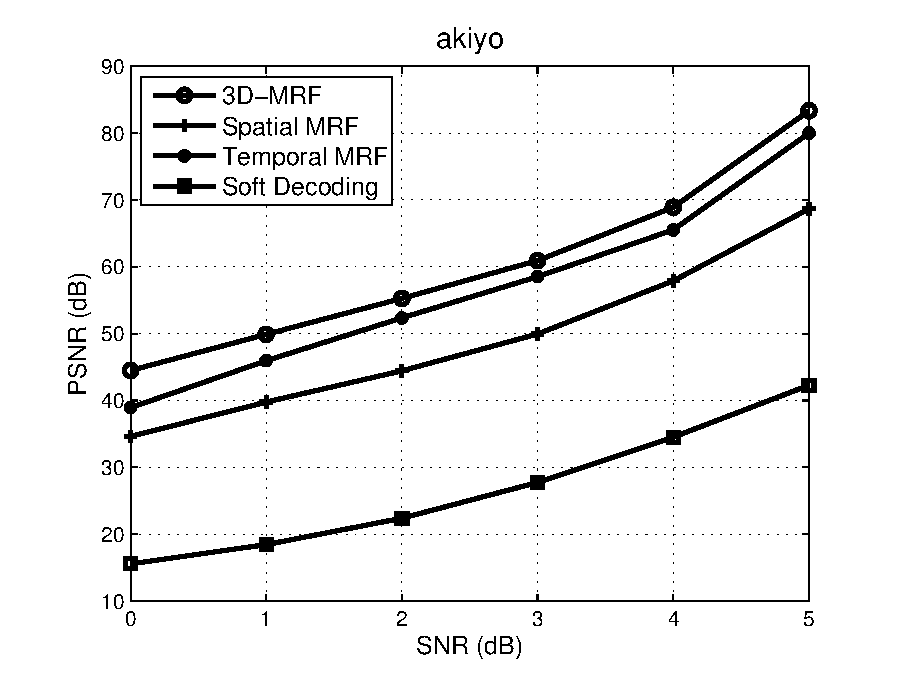
\includegraphics[width=0.45\textwidth]{./images/result/akiyo.eps}}
\subfloat[]{\label{fig_result_b}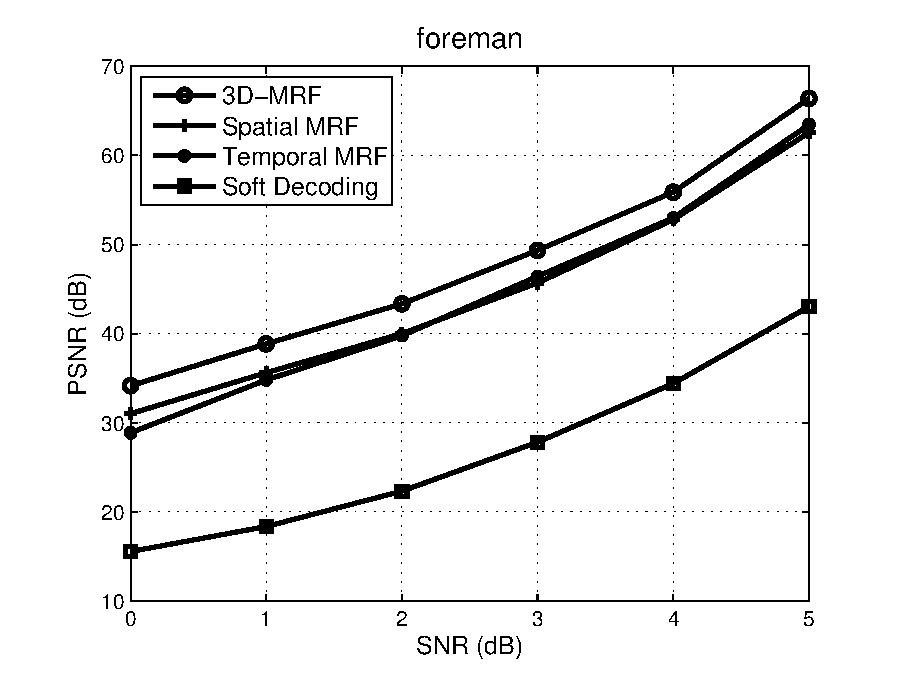
\includegraphics[width=0.45\textwidth]{./images/result/foreman.eps}}\\
\subfloat[]{\label{fig_result_c}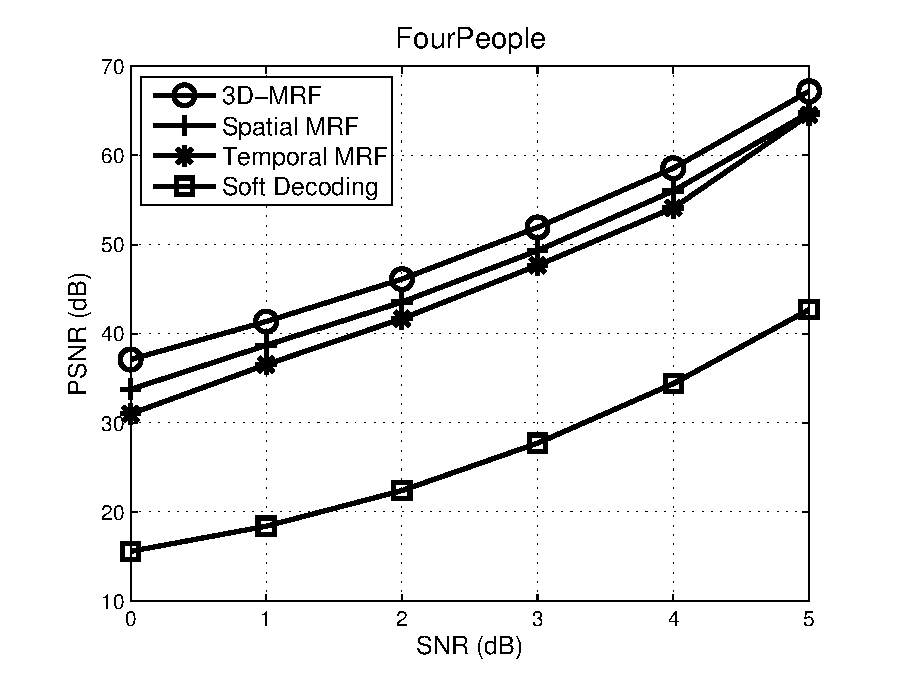
\includegraphics[width=0.45\textwidth]{./images/result/fourpeople.eps}}
\subfloat[]{\label{fig_result_d}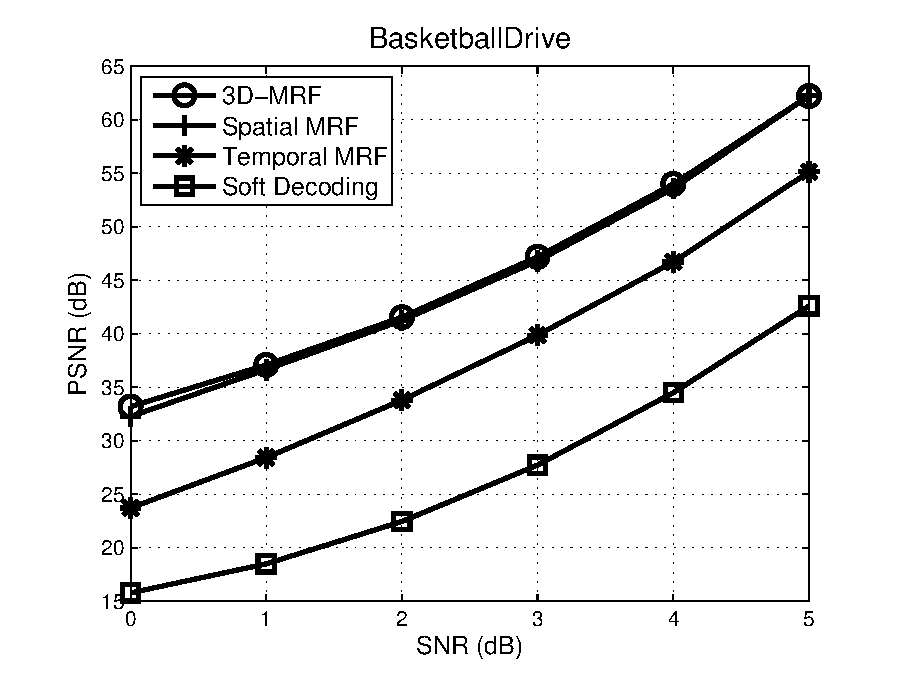
\includegraphics[width=0.45\textwidth]{./images/result/basketballdrive.eps}}
\caption{PSNR gain of proposed decoding method based on 3D-MRF model, where "Spatial MRF" and "Temporal MRF" denotes the decoding gain achieving by solely using the extrinsic information provided by the spatial and temporal decoder respectively, and "Soft decoding" is the BCJR decoding.}
\label{fig_result}
\end{figure*}

We evaluate the proposed iterative source-channel decoding by comparing the direct decoding of convolutional code with the decoder structures as shown in Fig. \ref{cf_de}. We use the recursive systematic convolution code which has the generator matrix 
\begin{align}
\mathbf{G}(D) &= \left[
\begin{array}{cc}
1 & \frac{1+D^2}{1+D+D^2}
\end{array} \right]
\label{cf_gnm} 
\end{align}
as the channel correction code, and two different random interleavers are used every other frame. The wireless signals are modulated by BPSK, and the channel noise is assumed to be AWGN. BCJR \cite{BCJR} is used as the soft-in soft-out channel decoder. The iteration count is set to br $3$ for all received frames. The evaluation metric is peak signal-to-noise ratio (PSNR). For a $8$-bit per pixel decoded video frame, the PSNR is represented as 
\begin{align}
PSNR = 20log_{10}({\frac{255}{\sqrt{\frac{1}{w\cdot h}\sum_{i=0}^{w\cdot h}{({f_i}-\hat{f_i})^2}}}}),
\end{align}
where $f_i$ is the pixel value of source video frame, and $\hat{f_i}$ is the decoded pixel value at the receiver. $w\cdot h$ is equal to the total number in a video frame.

We use four video sequences to test our proposed method. The test video sequences are composed of gray images, and $8$ bits are used to present a pixel. The first $30$ video frames are used to evaluate our proposed method. The first sequence is the ``akiyo" sequence with resolution $352x288$, in which the human facial expression and body movement present. The second sequence is the ``foreman" sequence with resolution $352x288$, where there is a camera pan movement and apparent facial expression. The third sequence is the ``FourPeople" sequence with resolution $1280x720$, in which the image detail of a conversation between four people is presented with higher resolution. The forth sequence is the ``BasketballDrive" sequence with resolution $1920x1080$, which presents the strongest camera movement and the highest video details in a basketball game. We select the last two video sequences in order to test the performance of our proposed scheme with different video resolutions, even for high-definition video contents. In summary, these four video sequences have the common video content, which can test our proposed method in an objective way.

The PSNR gain of our proposed scheme is significant as shown in Fig. \ref{fig_result}. It is because that the bit planes homogeneity is increasing from LSBs to MSBs, and the MSBs have the most significant influence on the perceptual qualities as well as PSNR while LSBs have the least. Therefore, the proposed decoding method benefits from the much better correction ability for the more important data. In other words, the UEP is achieved with the inherent image properties. Note that the proposed scheme can still cooperate with other conventional UEP to further improving the video quality. The PSNR gain in motionless video sequences such as ``akiyo" is greater than sequences with more movement such as ``BasketballDrive", since the former has much larger temporal redundancy than the latter one. Nevertheless, the PSNR gain provided by our decoding method for video sequence with intense movement is still quite apparent due to the decoder side motion estimation which exploits the temporal redundancy in these video sequences.

Also, it is worth noting that even in an extremely low SNR condition (e.g., 1 or 0), the PSNR gains generated by joint multi-frame decoding method
are all about 20dB higher than the original soft decoding even for the ``BasketballDrive" sequence, which has the strongest camera and object movement among our test video sequences. 

\section{Conclusion}\label{sec_con}
In this work, we have proposed an iterative source-channel decoding method for uncompressed video transmission based on our novel 3D-MRF model. By our proposed 3D-MRF model, one can describe the temporal and spatial redundancy in the transmitted video sequences in a simple bit-plane view. Firstly, based on the 3D-MRF model, we have developed the 3D-MRF based SISO source decoding algorithm which exploits the soft information in the received bit sequence without iterative process. Also, we estimate the 3D-MRF parameter at decoder side to automatically adjust the information shared between the decoded bit sequence without the aid from the encoder.  As a consequence, combing the source decoding and the parameter estimation of the 3D-MRF model, we have designed the iterative source-channel decoder scheme. In the proposed ISCD scheme, the extrinsic information is exchanged between the 3D-MRF source decoder and channel decoder, and we design a consecutive decoding structure which propagates the temporal information between video frames.

The numerical results have shown that our proposed method can significantly enhance the video quality in terms of PSNR for various video content and resolutions. Even when intense camera and object movement present, the PSNR gain is still quite remarkable. Furthermore, while the system is operating in an extremely low SNR condition, the video quality is still in good quality. As a result, our proposed scheme successfully enhances the quality and robustness of the wireless transmission of uncompressed video.

% use section* for acknowledgement
%\section*{Acknowledgment}


%The authors would like to thank...


% Can use something like this to put references on a page
% by themselves when using endfloat and the captionsoff option.
\ifCLASSOPTIONcaptionsoff
  \newpage
\fi



% trigger a \newpage just before the given reference
% number - used to balance the columns on the last page
% adjust value as needed - may need to be readjusted if
% the document is modified later
%\IEEEtriggeratref{8}
% The "triggered" command can be changed if desired:
%\IEEEtriggercmd{\enlargethispage{-5in}}

% references section

% can use a bibliography generated by BibTeX as a .bbl file
% BibTeX documentation can be easily obtained at:
% http://www.ctan.org/tex-archive/biblio/bibtex/contrib/doc/
% The IEEEtran BibTeX style support page is at:
% http://www.michaelshell.org/tex/ieeetran/bibtex/
\bibliographystyle{IEEEtran}
% argument is your BibTeX string definitions and bibliography database(s)
\bibliography{master_thesis_reference}
%
% <OR> manually copy in the resultant .bbl file
% set second argument of \begin to the number of references
% (used to reserve space for the reference number labels box)
%\begin{thebibliography}{1}
%
%\bibitem{IEEEhowto:kopka}
%H.~Kopka and P.~W. Daly, \emph{A Guide to \LaTeX}, 3rd~ed.\hskip 1em plus
%  0.5em minus 0.4em\relax Harlow, England: Addison-Wesley, 1999.
%
%\end{thebibliography}

% biography section
% 
% If you have an EPS/PDF photo (graphicx package needed) extra braces are
% needed around the contents of the optional argument to biography to prevent
% the LaTeX parser from getting confused when it sees the complicated
% \includegraphics command within an optional argument. (You could create
% your own custom macro containing the \includegraphics command to make things
% simpler here.)
%\begin{IEEEbiography}[{\includegraphics[width=1in,height=1.25in,clip,keepaspectratio]{mshell}}]{Michael Shell}
% or if you just want to reserve a space for a photo:

% You can push biographies down or up by placing
% a \vfill before or after them. The appropriate
% use of \vfill depends on what kind of text is
% on the last page and whether or not the columns
% are being equalized.

%\vfill

% Can be used to pull up biographies so that the bottom of the last one
% is flush with the other column.
%\enlargethispage{-5in}



% that's all folks
\end{document}


